\chapter[Differential Equations]{Models Defined by Systems
of Differential Equations}

\prologue{The universe is like a safe to which there is a combination,
but the combination is locked up in the safe.}{Peter de Vries}

An important class of models is that in which the responses are
described by a linear system of ordinary differential
\index{model!linear differential equations}
equations.
These models are used in chemical kinetics
\cite{from:bisc:1979} and in pharmacokinetics
%\glossary{ Froment, G.F.}
%\glossary{ Bischoff, K.B.}
\cite{godf:1983},
%\glossary{ Godfrey, K.}
where they are called {\em compartment\/} models.
\index{compartment model}
Because they are used in so many areas, it is worthwhile to have
special techniques to make their analysis easier.
Accordingly, in this chapter we present efficient methods for
estimating parameters in compartment models and for developing
and testing competing models.
Techniques for dealing with systems of nonlinear differential
equations are discussed in \citeasnoun{bard:1974} and
\citeasnoun{cara:stew:1985}.
%\glossary{ Bard, Y.}
%\glossary{ Caracotsios, M.}
%\glossary{ Stewart, W.E.}

\section{Compartment Models and System Diagrams}

A common use of compartment models is in pharmacokinetics,
where the exchange of materials
in biological systems is studied.
A system is divided into compartments, and
it is assumed that the rates of flow of drugs between
compartments follow first order kinetics, so that the rate of
transfer to a receiving, or {\em sink}, compartment is proportional
to the concentration in the supplying, or {\em source}, compartment.
\index{compartment model!sink}
\index{compartment model!source}
The transfer coefficients, which are assumed constant with respect to
time, are called {\em rate constants}.
\index{rate constant}

\begin{example}\label{tet:1}
  
As an example of a compartment model, we consider data on the
concentration of tetracycline hydrochloride in serum.  A
tetracycline compound was administered to a subject orally, and the
concentration of tetracycline hydrochloride in the serum was
measured over a period of 16 hours \cite{wagn:1967}.
The data are recorded in Appendix A, Section~\ref{atbl:tet},
and plotted in Figure \ref{fig:TETdata}.
\begin{figure}[tbp]
  \centerline{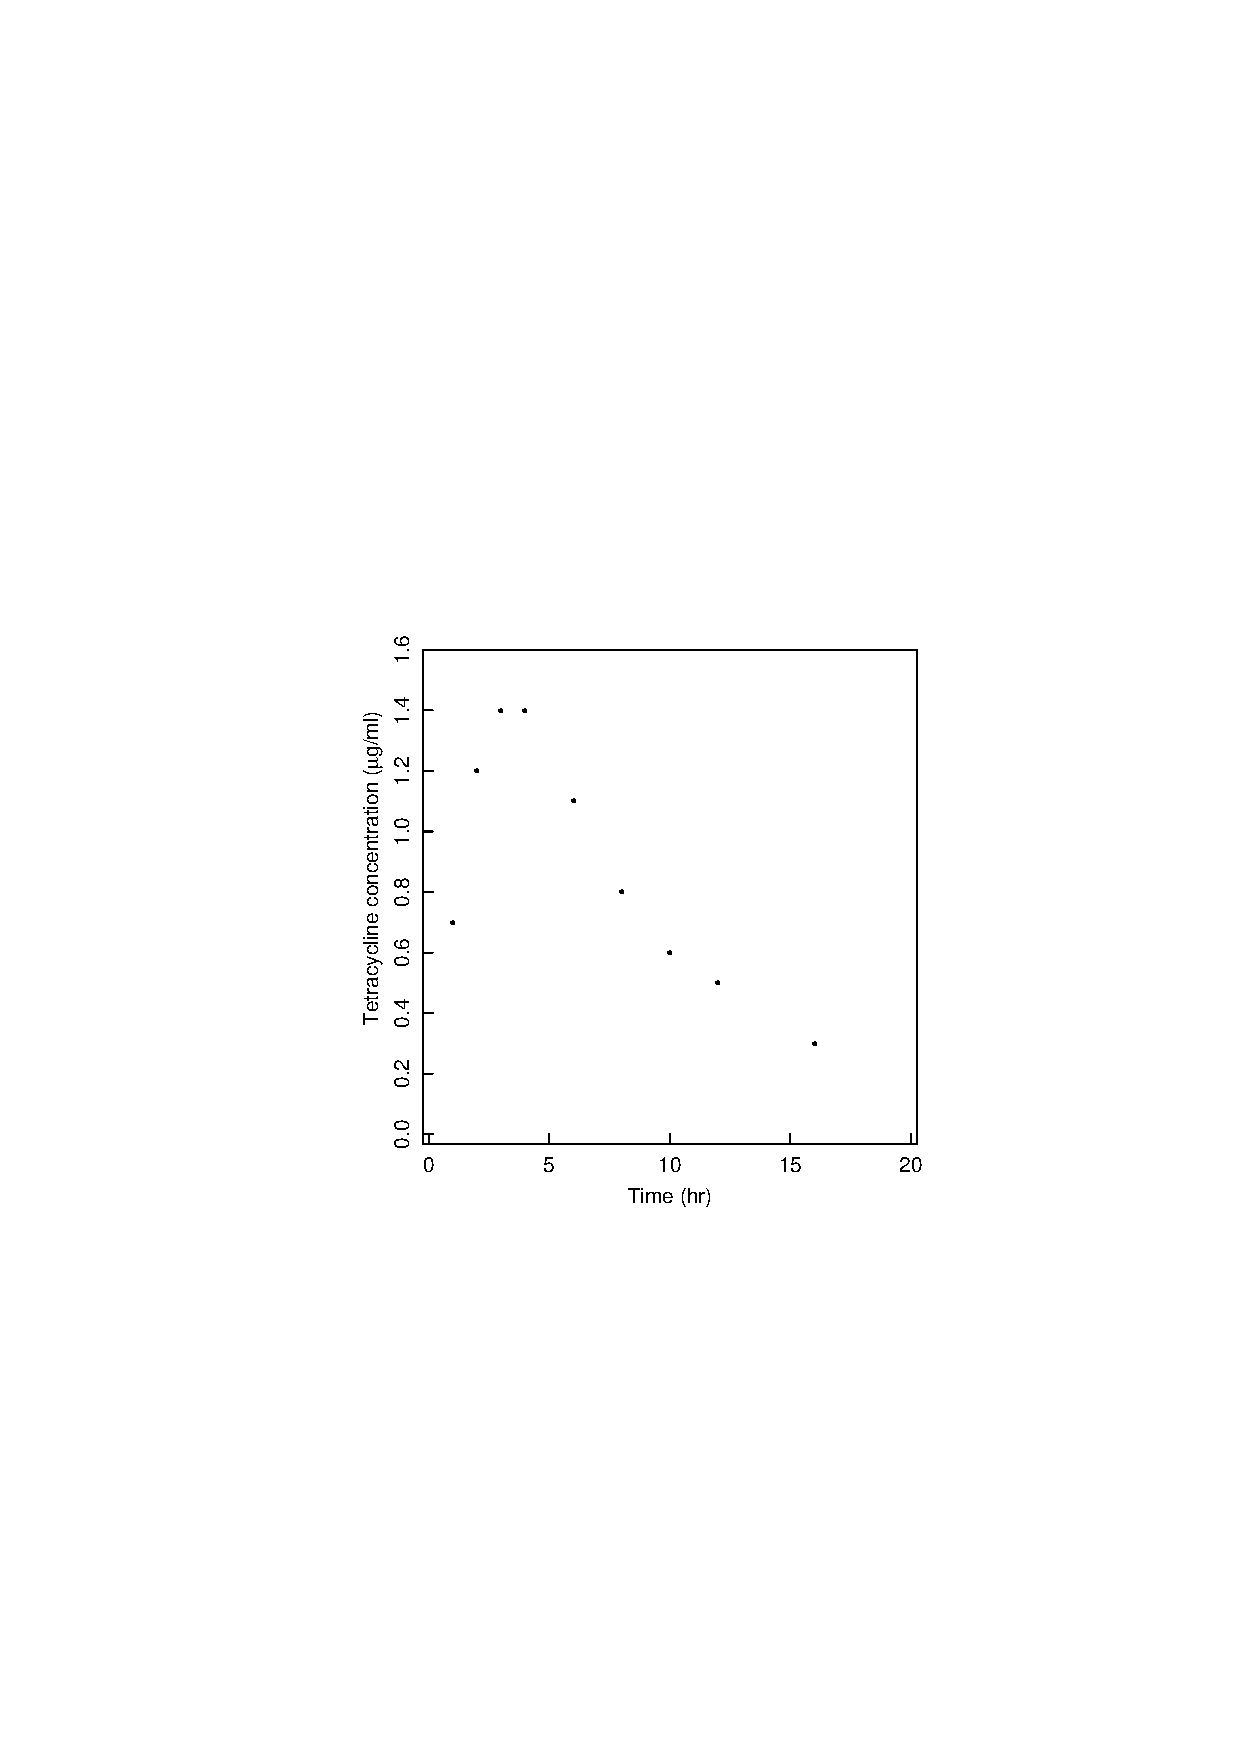
\includegraphics{5TETdata}}%,height=4in}}
  \caption{\label{fig:TETdata}
  Plot of tetracycline concentration versus time.}
\end{figure}


The biological system can be modeled by a gut compartment into
which the chemical is introduced, a blood compartment which
absorbs the chemical from the gut, and an elimination path.
Assuming first order kinetics, the concentrations
$( \gamma_1 (t) , \gamma_2 (t) ) \trans$
of tetracycline hydrochloride in the two compartments
can be described by the following pair of differential equations:
\begin{eqnarray} \label{eqn:5.1}
  {d \gamma_1 ( t )   \over  d t }&=&
  \dot \gamma_1 = - \theta_1 \gamma_1 ( t )\\
  {d \gamma_2 ( t )   \over  d t }&=&
  \dot \gamma_2 =
  \theta_1 \gamma_1 ( t ) - \theta_2 \gamma_2 ( t )\nonumber
\end{eqnarray}
where the dot denotes differentiation with
respect to time.

The system can be represented graphically as a compartment or system
diagram as in Figure \ref{fig:tet}.
\index{system diagram}
\expandafter\ifx\csname graph\endcsname\relax \csname newbox\endcsname\graph\fi
\expandafter\ifx\csname graphtemp\endcsname\relax \csname newdimen\endcsname\graphtemp\fi
\setbox\graph=\vtop{\vskip 0pt\hbox{%
    \special{pn 8}%
    \special{ar 250 250 250 250 0 6.28319}%
    \graphtemp=.5ex\advance\graphtemp by 0.250in
    \rlap{\kern 0.250in\lower\graphtemp\hbox to 0pt{\hss $\gamma_{1}$\hss}}%
    \special{pa 500 250}%
    \special{pa 1000 250}%
    \special{fp}%
    \special{sh 1.000}%
    \special{pa 900 225}%
    \special{pa 1000 250}%
    \special{pa 900 275}%
    \special{pa 900 225}%
    \special{fp}%
    \graphtemp=\baselineskip\multiply\graphtemp by -1\divide\graphtemp by 2
    \advance\graphtemp by .5ex\advance\graphtemp by 0.250in
    \rlap{\kern 0.750in\lower\graphtemp\hbox to 0pt{\hss $\theta_{1}$\hss}}%
    \special{ar 1250 250 250 250 0 6.28319}%
    \graphtemp=.5ex\advance\graphtemp by 0.250in
    \rlap{\kern 1.250in\lower\graphtemp\hbox to 0pt{\hss $\gamma_{2}$\hss}}%
    \special{pa 1250 500}%
    \special{pa 1250 1000}%
    \special{fp}%
    \special{sh 1.000}%
    \special{pa 1275 900}%
    \special{pa 1250 1000}%
    \special{pa 1225 900}%
    \special{pa 1275 900}%
    \special{fp}%
    \graphtemp=.5ex\advance\graphtemp by 0.750in
    \rlap{\kern 1.250in\lower\graphtemp\hbox to 0pt{\hss $\theta_{2}$ }}%
    \hbox{\vrule depth1.000in width0pt height 0pt}%
    \kern 1.500in
  }%
}%

\begin{figure}
  \centerline{\box\graph}
  \caption{\label{fig:tet}
  A compartment or system diagram for the tetracycline model.}
\end{figure}
\end{example}

Chemical reactions can also be described by linear systems of first
order differential equations.
In this context, the chemical species
of the reaction constitute the compartments, the original species
being termed ``parents,''
and the product species ``daughters.''

\begin{example}\label{oil:1}

As a chemical example, we consider the pyrolysis of oil shale
described by \citeasnoun{zieg:gorm:1980}.
%\glossary{ Ziegel, E.R.}
%\glossary{ Gorman, J.W.}
Oil shale contains organic material which is organically bonded to the
structure of the rock.
To extract oil from the rock, heat is applied so the technique is
called pyrolysis.

During pyrolysis, the benzene organic material, called kerogen,
decomposes to oil and bitumen, and there are unmeasured by-products of
insoluble organic residues and light gases.
Ziegel and Gorman, using data obtained from
\citeasnoun{hubb:robi:1950}, estimated the rate constants in several
%\glossary{ Hubbard, A.B.}
%\glossary{ Robinson, W.E.}
candidate models.
The data obtained by Hubbard and Robinson are listed
in Appendix A, Section~\ref{atbl:oil}.

The final model fitted by Ziegel and Gorman to the 400$^\circ$C data
using multiresponse
estimation techniques can be represented by the system diagram
in Figure \ref{fig:ziggy},
which corresponds to the set of linear differential
equations,
\begin{eqnarray}\label{eqn:5.2}
  {d\gamma_1\over dt}&=&-(\theta_1+\theta_4)\gamma_1\\
  {d\gamma_2\over dt}&=&\theta_1\gamma_1-(\theta_2+\theta_3)\gamma_2\nonumber\\
  {d\gamma_3\over dt}&=&\theta_4\gamma_1+\theta_2\gamma_2\nonumber
\end{eqnarray}
In this equation, $\gamma_1$ denotes kerogen, $\gamma_{2}$
bitumen, and $\gamma_{3}$ oil.
\expandafter\ifx\csname graph\endcsname\relax \csname newbox\endcsname\graph\fi
\expandafter\ifx\csname graphtemp\endcsname\relax \csname newdimen\endcsname\graphtemp\fi
\setbox\graph=\vtop{\vskip 0pt\hbox{%
    \special{pn 8}%
    \special{ar 250 650 250 250 0 6.28319}%
    \graphtemp=.5ex\advance\graphtemp by 0.650in
    \rlap{\kern 0.250in\lower\graphtemp\hbox to 0pt{\hss $\gamma_{1}$\hss}}%
    \special{pa 500 650}%
    \special{pa 1000 650}%
    \special{fp}%
    \special{sh 1.000}%
    \special{pa 900 625}%
    \special{pa 1000 650}%
    \special{pa 900 675}%
    \special{pa 900 625}%
    \special{fp}%
    \graphtemp=\baselineskip\multiply\graphtemp by -1\divide\graphtemp by 2
    \advance\graphtemp by .5ex\advance\graphtemp by 0.650in
    \rlap{\kern 0.750in\lower\graphtemp\hbox to 0pt{\hss $\theta_{1}$\hss}}%
    \special{ar 1250 650 250 250 0 6.28319}%
    \graphtemp=.5ex\advance\graphtemp by 0.650in
    \rlap{\kern 1.250in\lower\graphtemp\hbox to 0pt{\hss $\gamma_{2}$\hss}}%
    \special{pa 1500 650}%
    \special{pa 2000 650}%
    \special{fp}%
    \special{sh 1.000}%
    \special{pa 1900 625}%
    \special{pa 2000 650}%
    \special{pa 1900 675}%
    \special{pa 1900 625}%
    \special{fp}%
    \graphtemp=\baselineskip\multiply\graphtemp by -1\divide\graphtemp by 2
    \advance\graphtemp by .5ex\advance\graphtemp by 0.650in
    \rlap{\kern 1.750in\lower\graphtemp\hbox to 0pt{\hss $\theta_{2}$\hss}}%
    \special{ar 2250 650 250 250 0 6.28319}%
    \graphtemp=.5ex\advance\graphtemp by 0.650in
    \rlap{\kern 2.250in\lower\graphtemp\hbox to 0pt{\hss $\gamma_{3}$\hss}}%
    \special{pa 1250 900}%
    \special{pa 1250 1400}%
    \special{fp}%
    \special{sh 1.000}%
    \special{pa 1275 1300}%
    \special{pa 1250 1400}%
    \special{pa 1225 1300}%
    \special{pa 1275 1300}%
    \special{fp}%
    \graphtemp=.5ex\advance\graphtemp by 1.150in
    \rlap{\kern 1.250in\lower\graphtemp\hbox to 0pt{\hss $\theta_{3}$ }}%
    \special{ar 1250 2132 2000 2000 -2.094395 -1.047198}%
    \special{sh 1.000}%
    \special{pa 2176 328}%
    \special{pa 2250 400}%
    \special{pa 2151 372}%
    \special{pa 2176 328}%
    \special{fp}%
    \graphtemp=.5ex\advance\graphtemp by 0.000in
    \rlap{\kern 1.250in\lower\graphtemp\hbox to 0pt{\hss $\theta_{4}$\hss}}%
    \hbox{\vrule depth1.400in width0pt height 0pt}%
    \kern 2.500in
  }%
}%

\begin{figure}
  \centerline{\box\graph}
  \caption{\label{fig:ziggy}
  System diagram for the oil shale pyrolysis model.}
\end{figure}

The model implies that kerogen decomposes to bitumen with rate
constant $\theta_{1}$ and to oil with rate constant
$\theta_{4}$, and that bitumen decomposes to oil with rate constant
$\theta_{2}$ and to unmeasured by-products with rate constant
$\theta_{3}$.
\end{example}

In the general compartment model consisting of $K$ compartments,
we write the concentrations at time $t$ as
$\bgamma(t)=(\gamma_1(t),\ldots,\gamma_K(t))\trans$.
Assuming first order kinetics with rate constants
$\theta_1,\theta_2,\ldots,\theta_P$,
the concentrations obey the linear system of differential
equations
\begin{equation}
  \label{eqn:5.3}
  {d\bgamma\over dt}=\dot{\bgamma}(t)=\bA\bgamma(t)+\biota(t)
\end{equation}
where $\bA$ is the $K \times K$ system {\em transfer matrix\/}
\index{matrix!system transfer}
\index{transfer matrix}
containing the rate constants and $\biota(t)$ is a vector
function representing input to the system.

Although more complicated inputs may be used \cite{bate:wolf:watt:1986},
%\glossary{ Bates, D.M.}
%\glossary{ Wolf, D.A.}
%\glossary{ Watts, D.G.}
in this book we consider only two input functions.
One is a continuous infusion of material or {\em step input\/}
into the system,
$$
\biota ( t ) = \left\{
\begin{array}{c c}
  \biota&t\ge 0\\
  0&t<0
\end{array}
\right.
$$
where $\biota$ is a constant vector.
The other is a bolus or instantaneous injection, and although it
can be considered as an impulse or Dirac $\delta$-function input, it
is simpler to consider it as determining a vector of initial conditions
$\bgamma(0)=\bgamma_{0}$.

\begin{example}\label{tet:2}

For the tetracycline example, the input is a bolus in the gut,
and the transfer matrix $\bA$ can be readily obtained by
inspection of the differential equations (\ref{eqn:5.1}) or from the system
diagram (Figure \ref{fig:tet}), as
$$
\bA = \left[
\begin{array}{r r}
  -\theta_1&0\\
  \theta_1&-\theta_2
\end{array}
\right]
$$
The initial concentration of tetracycline hydrochloride in
the gut is unknown, but the concentration in the serum is assumed to be
zero, so we incorporate another parameter $\theta_{3}$ and
write $\bgamma_0=(\theta_3,0)\trans$.
\end{example}

\begin{example}\label{oil:2}

For the model (\ref{eqn:5.2}) suggested by \citeasnoun{zieg:gorm:1980},
%\glossary{ Ziegel, E.R.}
%\glossary{ Gorman, J.W.}
$$
\bA = \left[ \matrix {
\matrix { { - \theta_1 - \theta_4 } \cr \theta_1 \cr \theta_4 }
\matrix { 0 \cr { - \theta_2 - \theta_3 } \cr \theta_2 }
\matrix { 0 \cr 0 \cr 0 }
}\right]
$$
The recorded measurements for bitumen and oil are percentages of
the initial amount of kerogen, so we take
$\bgamma_0=(100,0,0)\trans$.
\citeasnoun{zieg:gorm:1980} found it necessary to incorporate
%\glossary{ Ziegel, E.R.}
%\glossary{ Gorman, J.W.}
a fifth parameter in the model to account for the unknown dead
time before the reaction began.
\end{example}

\section{Estimating Parameters in Compartment Models}

Several methods can be used to estimate parameters in compartment
models.
The most obvious is to obtain the analytic solution to
the system of differential equations and then use
the expectation function corresponding to the compartment
for which data are available
in a standard nonlinear estimation program.
A second approach is to use a standard nonlinear estimation
program, but calculate the function by solving the equations using
numerical integration.
A third approach \cite{ande:1983} is to recognize that the
%\glossary{ Anderson, D.H.}
responses $\gamma_1 ,  \gamma_2 ,\ldots, \gamma_{K}$
generally consist of
weighted sums of exponential functions of time, with the
exponents related to the system rate constants $\btheta$.
One can then fit a general sum of exponentials model and derive
estimates for the rate constants and other parameters.
This is not efficient, especially when the fitting is done
using the process of {\em peeling\/} (see Sections 3.3 and 3.9).
A fourth and superior {\em matrix exponential\/} approach,
\index{matrix!exponential}
proposed by \citeasnoun{jenn:brig:1976}, generates the
%\glossary{ Jennrich, R.I.}
%\glossary{ Bright, P.B.}
solution to the system of equations by
calculating values for the model function $\bgamma ( t )$ and its
derivatives directly, given values of $\btheta$, $t$, and
$\biota ( t )$.

The matrix exponential approach is
superior to the analytic solution approach because it avoids the
difficult and sometimes impossible task of deriving explicit
expressions for the model function and its derivatives.
In addition, it is possible to obtain the derivatives with
respect to the parameters in the same way as the expectation
function itself.
It is superior to the numerical integration approach
because it is faster and more accurate.
And finally,
it is superior to the sum of exponentials approach because
it avoids having to solve for the rate constants in terms of the
exponent and weight coefficients, and because the correct number of
parameters is incorporated directly into the model.

In the matrix exponential approach, if only one compartment is
observed, the expectation function $ f(t,\btheta)$ is simply the
appropriate element of the vector $ \bgamma(t)$,
and, as discussed in Section 4.3.4,
the function and its derivatives can
be obtained from the general solution by multiplying the expected
response matrix $\bH$, and the derivative of the expected response matrix
with respect to the parameters, by a $K \times1$ vector which is 0
except for a 1 in the appropriate row.
For example, for the tetracycline data, the concentration of
tetracycline hydrochloride in the serum is measured, and so
$\boeta = \bgamma_{2}$;  this response is therefore used in
estimating $\theta_{1}$ and $\theta_{2}$, and the expected response
matrix is multiplied by the vector $(0,1)\trans$.
In the oil shale example, oil and bitumen concentrations are
available, and so the multiresponse expectation matrix
$\bH=(\bgamma_2,\bgamma_3)$ can be used to estimate
the system parameters using the methods discussed
in Chapter 4.
In this case, the expected responses and their derivatives with respect
to the parameters will be multiplied by the $3\times2$
rotation matrix $\bB$, which consists of a row of zeros stacked above a
$2\times2$ identity matrix.

\subsection{Solving Systems of Linear Differential Equations}

The general solution to (\ref{eqn:5.3}) can be written
$$\label{eqn:5.4}
\bgamma ( t ) = e^{ \bA t } \bgamma_0
+ e^{ \bA t } * \biota ( t )
$$
where the matrix exponential
\index{matrix!exponential}
$e^{ \bA t }$ represents the convergent power series
$$\label{eqn:5.6}
e^{ \bA t } = \bI + {\bA t   \over  1 ! } +
{( \bA t )^2   \over  2 ! } +\cdots
$$
and the $*$ denotes convolution,
\index{convolution}
$$\label{eqn:5.5}
e^{ \bA t } * \biota ( t ) = \int_0^t
e^{ \bA ( t - u ) } \biota ( u )du
$$
The vector function is integrated componentwise.

Suppose $\bA$ is {\em diagonalizable}, so
\index{transfer matrix!diagonalizable}
there is a nonsingular matrix of eigenvectors, $\bU$, and
a diagonal matrix of eigenvalues,
\index{eigenvalue}
\index{eigenvector}
$\bLAMBDA ={\rm diag}(\lambda_1,\ldots,\lambda_K)$, such that
$$
\bA = \bU \bLAMBDA \bU^{-1}
$$
Then
$$
e^{{\bA} t} = \bU e^{{\bLAMBDA} t} \bU^{-1}
$$
with
$$
e^{{\bLAMBDA} t} ={\rm diag} ( e^{{\lambda}_1 t} ,\ldots,e^{{\lambda}_K t} )
$$
General computational methods for evaluating the convolution integral are
given in Appendix 5, and pseudocode is given in Appendix 3.

To develop the matrix exponential solution, we consider the special
situation in which $\bA$ is diagonalizable and the
input is a bolus, so the system (\ref{eqn:5.3}) can be written
$$\label{eqn:bolus}
\dot{\bgamma}  =  \bA \bgamma  t    0
$$
$$
\bgamma ( 0 )   =  \bgamma_0
$$
Then (\ref{eqn:bolus}) becomes
\begin{eqnarray}
  \dot{\bgamma}&=&\bA\bgamma  \\
  &=& \bU \bLAMBDA \bU^{-1} \bgamma
\end{eqnarray}
Premultiplying both sides of the equation by $\bU^{-1}$, and
letting $\bxi = \bU^{-1} \bgamma$, gives
$$
\dot{\bxi}= \bLAMBDA \bxi
$$
which is a set of independent first order differential
equations
$$
\dot{\xi}_k = \lambda_k \xi_k k = 1 , 2 ,\ldots, K
$$
with solutions
$$
\xi_k ( t )=e^{{\lambda}_k t }\xi_k ( 0 )
$$
where $\xi_k ( 0 )$ is the $k$th element of
$\bU^{-1} \bgamma_0 $.
Reverting to $\bgamma = \bU \bxi$ gives
$$\label{eqn:ebolus}
\bgamma ( t ) = \bU e^{{\bLAMBDA} t} \bU^{-1} \bgamma_0
 = e^{ \bA t } \bgamma_0
$$
Thus, for a bolus or impulse input, the convolution integral
(\ref{eqn:5.5}) reduces to (\ref{eqn:ebolus}).
\begin{example}\label{tet:3}
For the tetracycline example,
$\bgamma_0 = ( \theta_3 ,  0) \trans$, and
$$\label{eqn:5.7}
\bA = \left[ \matrix {
\matrix {- \theta_1 \cr \theta_1 }
\matrix { 0 \cr - \theta_2 }
}\right]
$$
For this simple system, we can calculate
eigenvalues and eigenvectors of the transfer matrix (\ref{eqn:5.7})
and use these to obtain explicit analytic expressions for
the responses.
Thus,
$$
\bLAMBDA = \left[ \matrix {
  \matrix{ - \theta_1 \cr 0}
  \matrix{ 0 \cr - \theta_2}
}\right]
$$
and
$$
\bU = \left[ \matrix {
\matrix { 1 \cr { { \theta_1   \over  \theta_2 - \theta_1 } } }
\matrix { 0 \cr - \theta_1 }
}\right]
$$
so
$$
\bU^{-1} = \left[ \matrix {
\matrix { 1 \cr { {1 \over  \theta_2 - \theta_1 } } }
\matrix { 0 \cr - {1 \over \theta_1} }
}\right]
$$
and, using (\ref{eqn:ebolus}), the responses are
$$
\bgamma = \left[ \matrix {
\matrix { \theta_3 e^{ - \theta_1 t } \cr
   { { \theta_3 \theta_1 ( e^{ - \theta_1 t }
      - e^{ - \theta_2 t } )   \over  \theta_2 - \theta_1 } }
   }
}\right]
$$
\end{example}

\subsection*{Dead Time}
\index{dead time}

For the oil shale data, it was noted that the
system does not respond immediately to the input, so a
``dead time,''
$t_{0}$, must be incorporated into the model.
We then modify (\ref{eqn:5.3}) to
\begin{eqnarray}\label{eqn:dead}
  \dot{\bgamma}( \tau )&=&\bA \bgamma ( \tau ) + \biota ( \tau )\\
  \bgamma(0)&=&\bgamma_0
\end{eqnarray}
where $\tau = ( t - t_0 )_{+}$, that is,
$$
\tau = \left\{\begin{array}{l l}
t - t_0&t > t_0\\
0&t\le t_0
\end{array}\right.
$$
where $t_0$ can be known or unknown.
The general solution is then
$$\label{eqn:deadtau}
\bgamma ( \tau ) = \left \{ \matrix
   { \bgamma_0 \cr e^{ \bA \tau } \bgamma_0
          + e^{ \bA \tau }  * \biota ( \tau )}
  \matrix {\tau\le 0 \cr \tau = 0}\right .
$$

\begin{example}\label{tet:deadtime}

The tetracycline data also shows evidence of dead time in the
system.
Fitting the model (\ref{eqn:5.1}) gives the parameter estimates in
Table~\ref{tbl:tetest1}.
\begin{table}
  \begin{center}
    \caption{\label{tbl:tetest1}
      Parameter summary for the tetracycline model without dead time.
      }
    \begin{tabular}{clcllll} \hline
      &&\multicolumn{5}{c}{Logarithm Scale}\\ 
      &&& \multicolumn{1}{c}{Std.} & \multicolumn{3}{c}{Correlation}\\
      \multicolumn{1}{c}{Parameter} &\multicolumn{1}{c}{Value} &
      \multicolumn{1}{c}{$ln\theta $} & \multicolumn{1}{c}{Error} &
      \multicolumn{3}{c}{Matrix}\\ \hline
      $\theta_{1}$&0.1830&--1.698&0.244&1.00\\
      $\theta_{2}$&0.4345&--\/0.8335&0.272&--\/0.96&1.00\\
      $\gamma_1 ( 0 )$&5.996&1.791&0.318&--\/0.98&0.99&1.00\\ \hline
    \end{tabular}
  \end{center}
\end{table}
A plot of the data and the fitted response versus time, in
Figure~\ref{fig:TETest1}, shows a poor fit, since the fitted curve is too
squat.
\begin{figure}
  \centerline{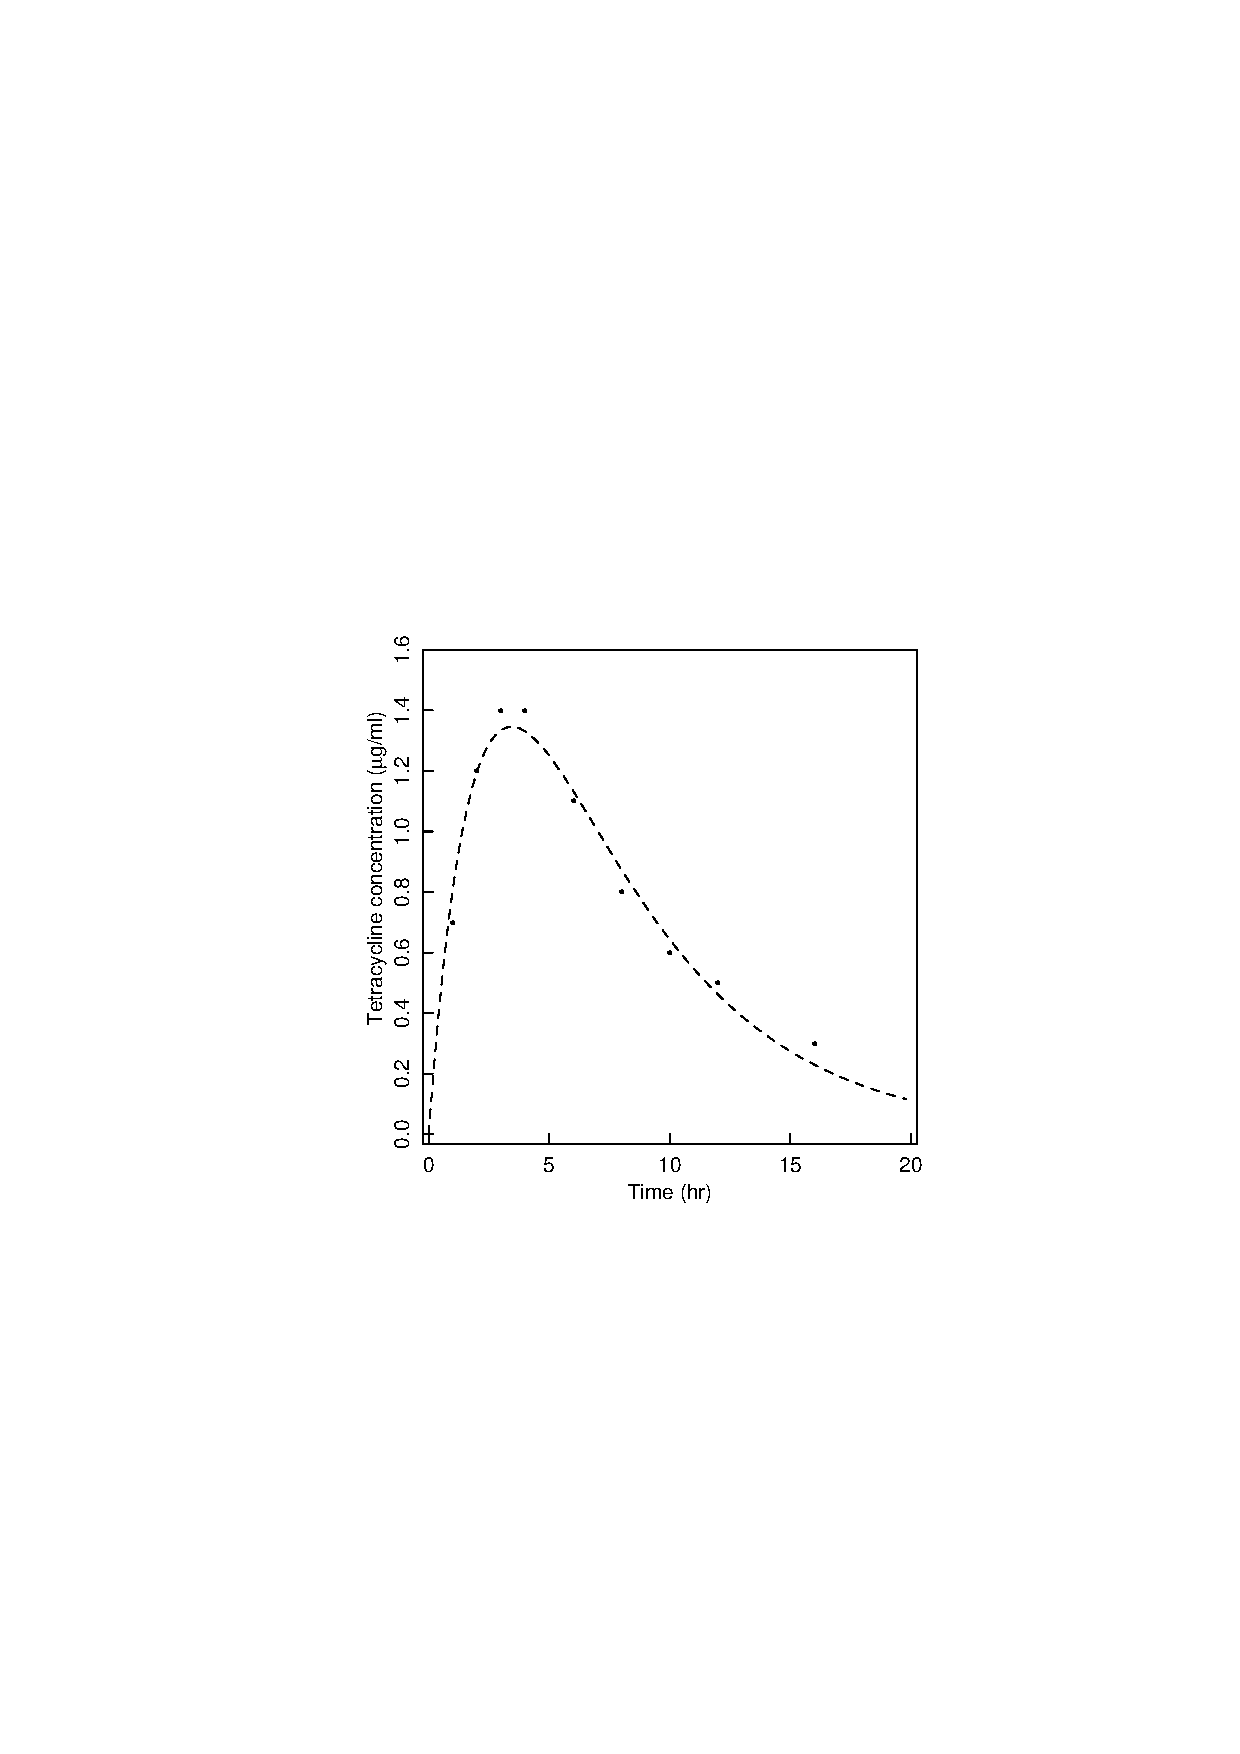
\includegraphics{5TETest1}}%,height=4in}}
  \caption{\label{fig:TETest1}
  Plot of the tetracycline data and the fitted response curve for the model
  without dead time.
  }
\end{figure}

Allowing for dead time with a fourth parameter produces
the estimates in
Table~\ref{tbl:tetest2} and the fitted curve plotted in
Figure~\ref{fig:TETest2}.
\begin{table}
  \begin{center}
    \caption{\label{tbl:tetest2}
      Parameter summary for the tetracycline model with dead time.
      }
    \begin{tabular}{c r r r r r r r} \hline
%c c c s s s s s
%c c c s s s s s
%c c c c c s s s
%c c c c c s s s
%c n n n n 1 n 1 n 1 n.
%\_
&&Logarithm Scale\\
%::
%:::Std.:Correlation
%Parameter:Value:$ln\theta $:Error:Matrix
%\par\vspace{2.0pt}
%\_
$\theta_{1}$&0.1488&--1.905&0.097&1.00\\
$\theta_{2}$&0.7158&--0.3343&0.176&--0.86&1.00\\
$\gamma_1 ( 0 )$&10.10&2.312&0.198&--0.92&0.99&1.00\\
$t_{0}$&0.4123&&0.095&--0.54&0.81&0.77&1.00\\ \hline
%\par\vspace{4.0pt}
%\_
    \end{tabular}
  \end{center}
\end{table}
\begin{figure}
  \centerline{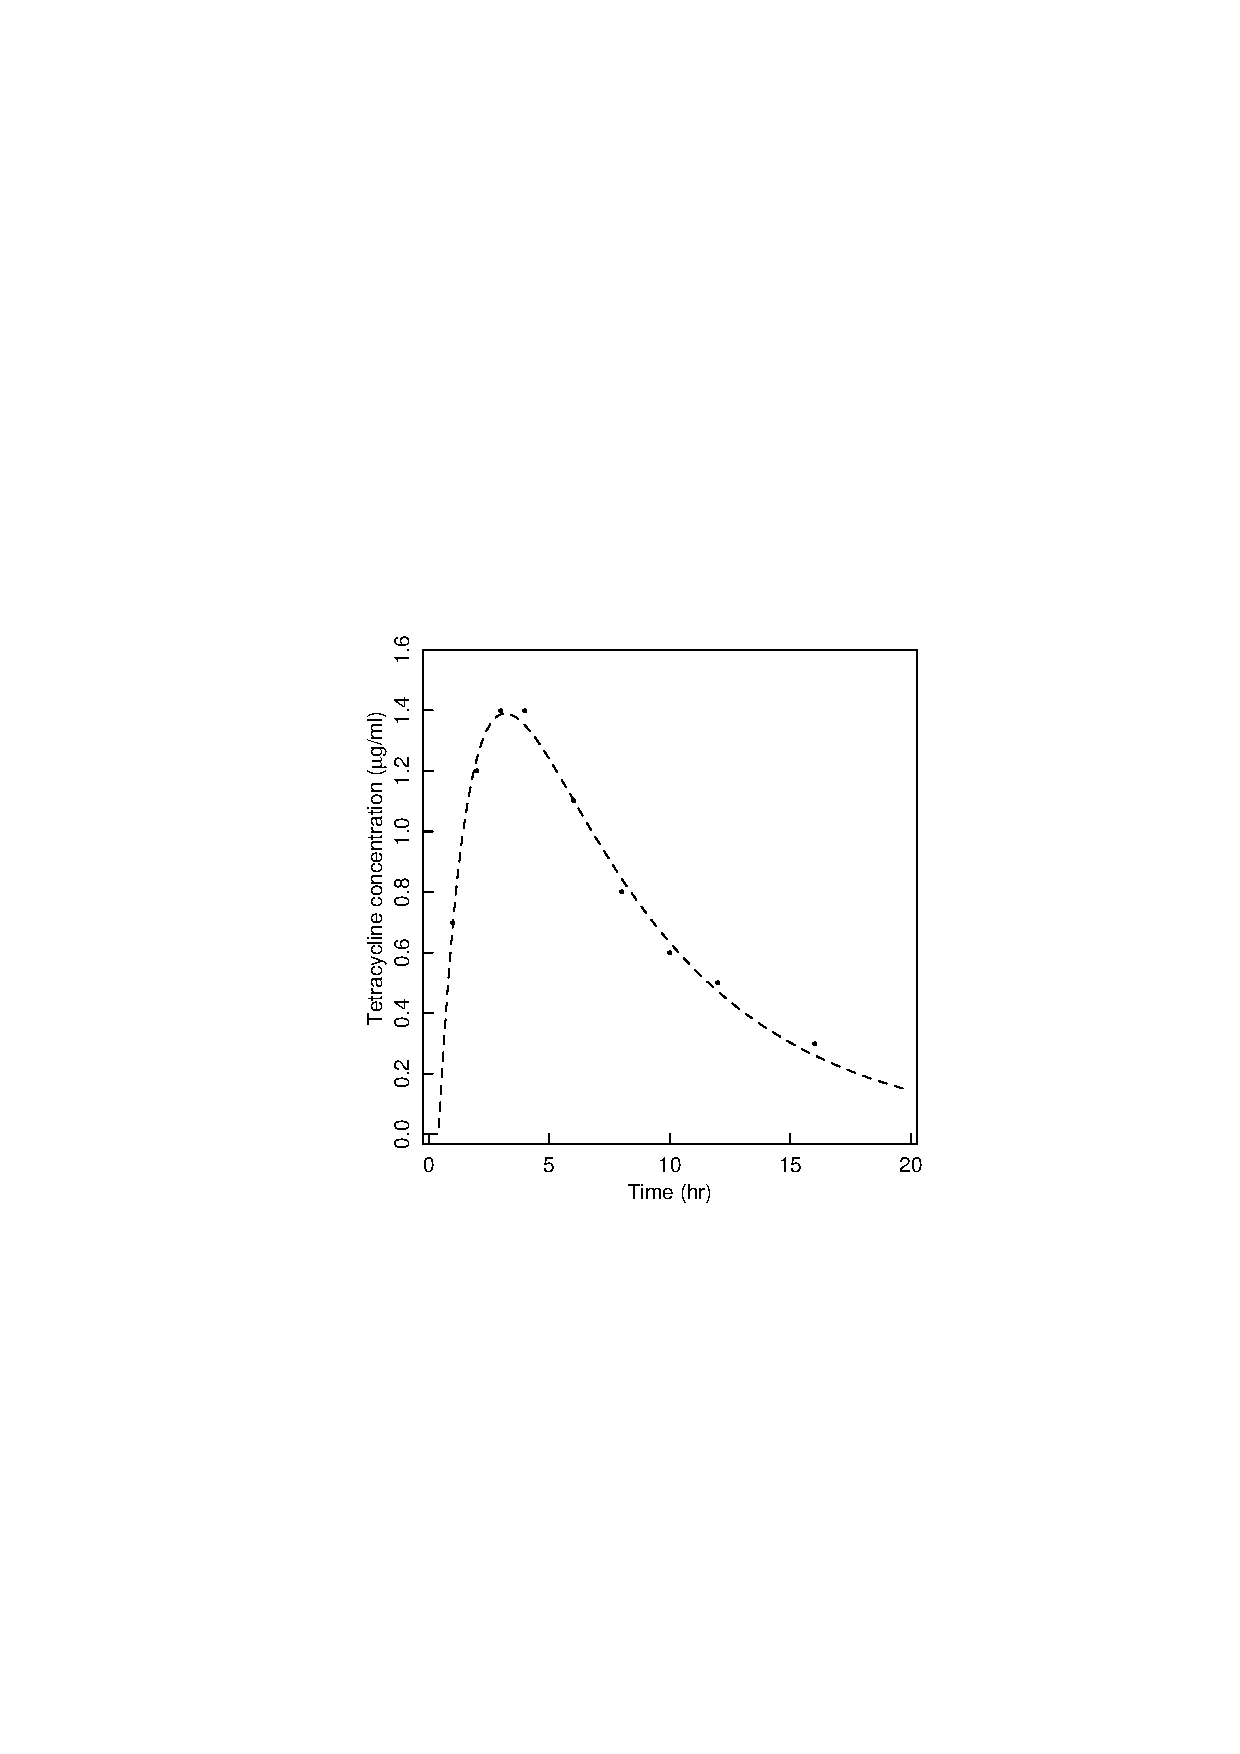
\includegraphics{5TETest2}}%,height=4in}}
  \caption{\label{fig:TETest2}
  Plot of the tetracycline data and the fitted response curve for the model
  with dead time.
  }
\end{figure}
This fit is better, especially for small time values.
An extra sum of squares analysis, as in
Table~\ref{tbl:tetlof}, confirms the need for dead time in the model.
\begin{table}
  \begin{center}
    \caption{\label{tbl:tetlof}
      Extra sum of squares analysis for dead time in the tetracycline model.
      }
    \begin{tabular}{c r r r r r r r}
%c c c c c c
%l c c c c c
%l n n n n n.
%\_
%:Sum of:Degrees of:Mean
%Source:Squares:Freedom:Square:F Ratio:$p$ Value
%\par\vspace{2.0pt}
%\_
Extra&0.02560&1&0.02560&12.736&0.016\\
4-parameter&0.01005&5&0.00201\\
%\par\vspace{2.0pt}
%\_
3-parameter&0.03565&6\\ \hline
%\par\vspace{2.0pt}
%\_
    \end{tabular}
  \end{center}
\end{table}
\end{example}

\subsection*{Cessation of Infusion}

With continuous infusion there is sometimes another critical time,
$t_{f}$, when the infusion is stopped.  In pharmacokinetic studies,
the period $0 t \le t_{f}$ is called the {\em on-infusion} stage, and
the period $t t_{f}$ is called the {\em off-infusion} stage.
If there are measurements in the off-infusion stage, the model
function during off-infusion, say $\bgamma_{{\rm off}} (t)$, is evaluated
by using the on-infusion model function
evaluated at $t_{f}$, as the initial condition vector
in a new system with $\biota =  {\bf 0} $.
Thus, assuming the initial conditions are zero, for the
on-infusion stage we have
$$
\bgamma_{{\rm on}} ( t ) = e^{ \bA t } * \biota ( t ) 
t \le t_f
$$
and for the off-infusion stage we have
$$
\bgamma_{{\rm off}} ( t ) =
e^{ \bA (t - t_f )} \bgamma_{{\rm on}} ( t_f ) 
t  t_f
$$

\subsection{Derivatives of the Expectation Function}
\index{derivative!compartment model}
\index{compartment model!derivative with respect to parameter}

To estimate the parameters using a Gauss--Newton procedure,
we must evaluate the derivatives with respect to the parameters.
As shown by \citeasnoun{jenn:brig:1976}, a great advantage of
%\glossary{ Jennrich, R.I.}
%\glossary{ Bright, P.B.}
systems of linear differential equations is that these derivatives can
be evaluated in the same manner as the model function itself.
They differentiated the general solution
(\ref{eqn:deadtau}) directly to get the gradient terms, but in
\citeasnoun{bate:watt:1985}, we
%\glossary{ Bates, D.M.}
%\glossary{ Watts, D.G.}
exploited the interchangability of differentiation with
respect to time and with respect to a parameter to generate another
set of linear system of differential equations which can be solved
directly.

As in Chapter 4, we use a subscript in parentheses to denote
differentiation with respect to a parameter and
write, for example,
$$
{ \partial \bgamma ( \tau )   \over  \partial \theta_p }  =
\bgamma_{(p)}p = 1 , 2 ,\ldots, P
$$
If only $\tau$ depends on $\theta_{p}$, the derivative of
$\bgamma ( \tau )$ with respect to
$\theta_{p}$ can be evaluated directly from
(\ref{eqn:dead}) using the chain rule, so
$$\label{eqn:taud}
\bgamma_{(p)} ( \tau ) = \tau_{(p)} [ \bA \bgamma ( \tau ) +
\biota ]
$$
When $\bA$, $\bgamma_{0}$, or $\biota$, but not $\tau$, depends on
$\theta_{p}$, we get the derivative
$\bgamma_{(p)} ( \tau )$ by differentiating (\ref{eqn:dead}) with
respect to $\theta_{p}$ to obtain
$$
\dot{\bgamma}_{(p)} ( \tau ) = \bA \bgamma_{(p)} ( \tau ) +
\bA_{(p)} \bgamma ( \tau ) + \biota_{(p)}
$$
This is simply another linear system of differential equations
with driving function $\bA_{(p)} \bgamma ( \tau ) + \biota_{(p)}$,
for which the solution is
\begin{eqnarray}
  \bgamma_{(p)}(\tau)&=&e^{ \bA \tau } \bgamma_{(p)} (0) +
  e^{ \bA \tau } * [ \bA_{(p)} \bgamma ( \tau ) + \biota_{(p)} ]\\
  &=& e^{ \bA \tau } \bgamma_{(p)} (0) +
  e^{ \bA \tau } * \biota_{(p)} +
  e^{ \bA \tau } * \bA_{(p)} e^{ \bA \tau } \bgamma_0  +
  e^{ \bA \tau } * \bA_{(p)} e^{ \bA \tau } * \biota
  \label{eqn:5.8}
\end{eqnarray}
To get a general expression for $\theta_{p}$ determining any
of $\tau$, $\bA$, $\bgamma_{0}$, and $\biota$,
we combine (\ref{eqn:5.8}) and (\ref{eqn:taud}) to give the expression
$$\label{eqn:alld}
\bgamma_{(p)} ( \tau ) = e^{ \bA \tau } \bgamma_{(p)} ( 0 )
+ e^{ \bA \tau } * [ \bA_{(p)} \bgamma ( \tau ) + \biota_{(p)} ]
+ \tau_{(p)} [ \bA \bgamma ( \tau ) + \biota ]
$$
which is true for an impulse or step input.

It is easy to evaluate $\bA_{(p)}$,
$\bgamma_{(p)} (0) = { \partial \bgamma_0 } / { \partial \theta_p}$,
$\biota_{(p)}$, and $\tau_{(p)}$, since the elements of the derivatives
are always --1, +1, or 0.

Note that the method can be extended to higher order derivatives:
in particular, the derivative with respect to
$\theta_{p}$ and $\theta_{q}$ is
$$\label{eqn:5.9}
\bgamma_{(pq)} ( \tau ) =
e^{ \bA \tau } * ( \bA_{(p)} \bgamma_{(q)} ( \tau ) ) +
e^{ \bA \tau } * ( \bA_{(q)} \bgamma_{(p)} ( \tau ) )
$$
since the elements of $\bA_{(pq)}$, $\bgamma_{(pq)} (0)$,
$\biota_{(pq)}$, and $\tau_{(pq)}$ are all 0.

\begin{example}\label{tet:4}

For the tetracycline example with delay time, we have
$\tau = ( t - \theta_4 )_{+}$,
$\bgamma_0 = ( \theta_3 ,  0 ) \trans$
and
$$
\bA = \left[ \matrix {
\matrix { - \theta_1 \cr \theta_1 }
\matrix { 0 \cr - \theta_2 }
}\right]
$$
so that
$$
\bA_{(1)} = \left[ \matrix {
\matrix { - 1 \cr 1 }
\matrix { 0 \cr 0 }
}\right] , 
\bA_{(2)} = \left[ \matrix {
\matrix { 0 \cr 0 }
\matrix { 0 \cr -1 }
}\right] , 
\bA_{(3)} = \bA_{(4)} = \left[ \matrix {
\matrix { 0 \cr 0 }
\matrix { 0 \cr 0 }
}\right]
$$
$$
\bgamma_{(1)} ( 0 ) = \bgamma_{(2)} ( 0 ) =
\bgamma_{(4)} ( 0 ) = \left[ \matrix {
\matrix { 0 \cr 0 }
}\right] , 
\bgamma_{(3)} ( 0 ) = \left[ \matrix {
\matrix { 1 \cr 0 }
}\right]
$$
$$
\tau_{(1)} = \tau_{(2)} = \tau_{(3)} = 0 , 
\tau_{(4)} = \left\{ \matrix { \matrix {-1 \cr 0}
\matrix { \tau \ge 0 \cr \tau  0}
}\right.
$$
and all second derivatives of these quantities are zero.
\end{example}

The functions $\bgamma_{(p)} ( \tau ),p=1 ,\ldots, P$,
are called the
%
{\em sensitivity functions }
of the system \cite{cara:stew:1985}
%\glossary{ Caracotsios, M.}
%\glossary{ Stewart, W.E.}
and can be evaluated
for any $\tau$ and $\btheta$ using (\ref{eqn:alld}) and the results
of Appendix 5.
Pseudocode for fitting compartment models is given in Appendix 3.

\section{Practical Considerations}
\index{practical considerations!compartment models}
\index{compartment model!practical considerations}

In this section we discuss some practical considerations related
to fitting compartment models.
\subsection{Parameter Transformations}
\index{parameter!transformation}
\index{transformation!of parameters}

A property of compartment models is that the rate
\index{rate constant}
constants, initial concentrations, and infusion rates must be
positive.
As discussed in Section 3.4, an effective way to ensure
positive values is to use logarithms of the parameters in the model.
This also enables linear approximation inference intervals
for some important derived quantities to be obtained easily.

For example, the {\em half-life}, $t_{{1/2}}$, associated with the
\index{half-life}
rate constant $\theta$ is $\ln2 / \theta  \approx  0.693 / \theta$.
Then
\begin{eqnarray}
\ln t_{{1/2}}&=&\ln\ln2  - \ln\theta\\
&\approx&-0.367 - \ln\theta
\end{eqnarray}
and the width of a linear approximation inference interval for
$\ln t_{{1/2}}$ is the same as the width of the
interval for $\ln\theta $.

Another derived quantity of interest in pharmacological studies
is the %
{\em volume of distribution }
in a compartment.
\index{volume of distribution}
With a bolus injection, the dose, say $D$, in the initial
compartment is known, but the concentration $\gamma_0 $ is
estimated.
These are related by
$$
\gamma_0 = { D   \over  V_i }
$$
where $V_{i}$ is the volume of distribution for the injection
compartment.
Again, the logarithms of $\gamma_0 $ and $V_{i}$ are
linearly related,
$\ln V_i =\ln D -\ln\gamma_0 $,
and linear approximation confidence intervals on the logarithms have
the same width.

A third derived quantity of interest in pharmacological studies is
the {\em area under the curve\/} (AUC).
\index{AUC (area under the curve)}
For many simple compartment models this is equal to the initial
concentration in the injection compartment, say $\gamma_1 ( 0 )$,
divided by the elimination rate, say $\theta_{1}$, so
AUC$ = { \gamma_1 ( 0 )} / {\theta_1}$.
Again, $\ln\mbox{AUC}$  is linearly related to $\ln\gamma_1 ( 0 ) $ and
$\ln\theta_1 $, so linear approximation confidence intervals for
$\ln\mbox{AUC}$ are easily calculated.

In chemical kinetics, sometimes data are collected
under different experimental conditions, and the analyst would
like to combine the data in order to fit a more general model,
as discussed in Section 3.11 and demonstrated in Section 5.5.
In these cases, it is often assumed that the rate constants
depend on the absolute temperature $T$ according to an Arrhenius
\index{Arrhenius relation}
relation ($\theta \propto e^{-k/T} $) multiplied by products of
pressures $P_{i}$ raised to powers.
For these models, the logarithms of the rate constants are
linear functions of $1/T$ and $\ln P_i$,
which provides another rationale for using logarithms.

An apparent disadvantage of using logarithms is that we cannot use
linear approximation inference intervals to indicate whether a
parameter could be zero, because they
will never contain points corresponding to zero.
However, a logarithm which is tending to a large negative value
suggests that the parameter might be zero, and by using the matrix
exponential method it is
straightforward to eliminate that path or term in the compartment model,
and then compare the reduced model with the original model using an
extra sum of squares analysis.
Besides, as explained in Section 3.10, the extra sum of squares test
is more valid than the approximate $t$ test for nonlinear
regression.

\subsection{Identifiability}
\index{practical considerations!unidentifiable model}

A problem in fitting compartment models
{\em when only one response is observed\/}
is that some configurations result in exchangable parameters.
\index{parameter!exchangeable.}
This can cause problems in estimation,
as mentioned in Section 3.4.1, because
discrete sets of parameters give the same predicted responses.
The parameters in such models are said to be {\em locally\/}
identifiable rather than {\em globally\/} (uniquely)
identifiable \cite{godf:1983}.
%\glossary{ Godfrey, K.}
For example, in the system of
Figure~\ref{fig:abc} with $\bgamma_{0=(1,0,0)} \trans$,
the same $\gamma_3 ( t )$ curve results
for the parameter pair $( a ,  b )$ as for
$( b ,  a )$, so when only the third compartment is
measured, the parameters $\theta_{1}$ and $\theta_{2}$ are
exchangable.
\expandafter\ifx\csname graph\endcsname\relax \csname newbox\endcsname\graph\fi
\expandafter\ifx\csname graphtemp\endcsname\relax \csname newdimen\endcsname\graphtemp\fi
\setbox\graph=\vtop{\vskip 0pt\hbox{%
    \special{pn 8}%
    \special{ar 250 250 250 250 0 6.28319}%
    \graphtemp=.5ex\advance\graphtemp by 0.250in
    \rlap{\kern 0.250in\lower\graphtemp\hbox to 0pt{\hss $\gamma_{1}$\hss}}%
    \special{pa 500 250}%
    \special{pa 1000 250}%
    \special{fp}%
    \special{sh 1.000}%
    \special{pa 900 225}%
    \special{pa 1000 250}%
    \special{pa 900 275}%
    \special{pa 900 225}%
    \special{fp}%
    \graphtemp=\baselineskip\multiply\graphtemp by -1\divide\graphtemp by 2
    \advance\graphtemp by .5ex\advance\graphtemp by 0.250in
    \rlap{\kern 0.750in\lower\graphtemp\hbox to 0pt{\hss $\theta_{1}$\hss}}%
    \special{ar 1250 250 250 250 0 6.28319}%
    \graphtemp=.5ex\advance\graphtemp by 0.250in
    \rlap{\kern 1.250in\lower\graphtemp\hbox to 0pt{\hss $\gamma_{2}$\hss}}%
    \special{pa 1500 250}%
    \special{pa 2000 250}%
    \special{fp}%
    \special{sh 1.000}%
    \special{pa 1900 225}%
    \special{pa 2000 250}%
    \special{pa 1900 275}%
    \special{pa 1900 225}%
    \special{fp}%
    \graphtemp=\baselineskip\multiply\graphtemp by -1\divide\graphtemp by 2
    \advance\graphtemp by .5ex\advance\graphtemp by 0.250in
    \rlap{\kern 1.750in\lower\graphtemp\hbox to 0pt{\hss $\theta_{2}$\hss}}%
    \special{ar 2250 250 250 250 0 6.28319}%
    \graphtemp=.5ex\advance\graphtemp by 0.250in
    \rlap{\kern 2.250in\lower\graphtemp\hbox to 0pt{\hss $\gamma_{3}$\hss}}%
    \hbox{\vrule depth0.500in width0pt height 0pt}%
    \kern 2.500in
  }%
}%
    

\begin{figure}
  \centerline{\box\graph}
  \caption{\label{fig:abc}
  A system which has exchangable parameters when only $\gamma_{3}$ is observed.
  }
\end{figure}

A worse problem, though, is {\em unidentifiable\/}
models, where continuous {\em sets\/} of parameters
\index{model!unidentifiable}
\index{compartment model!unidentifiable}
give the same predictions.
For example, the system of
\expandafter\ifx\csname graph\endcsname\relax \csname newbox\endcsname\graph\fi
\expandafter\ifx\csname graphtemp\endcsname\relax \csname newdimen\endcsname\graphtemp\fi
\setbox\graph=\vtop{\vskip 0pt\hbox{%
    \special{pn 8}%
    \special{ar 250 250 250 250 0 6.28319}%
    \graphtemp=.5ex\advance\graphtemp by 0.250in
    \rlap{\kern 0.250in\lower\graphtemp\hbox to 0pt{\hss $\gamma_{1}$\hss}}%
    \special{ar 1250 250 250 250 0 6.28319}%
    \graphtemp=.5ex\advance\graphtemp by 0.250in
    \rlap{\kern 1.250in\lower\graphtemp\hbox to 0pt{\hss $\gamma_{2}$\hss}}%
    \special{pa 427 73}%
    \special{pa 1073 73}%
    \special{fp}%
    \special{sh 1.000}%
    \special{pa 973 48}%
    \special{pa 1073 73}%
    \special{pa 973 98}%
    \special{pa 973 48}%
    \special{fp}%
    \graphtemp=\baselineskip\multiply\graphtemp by -1\divide\graphtemp by 2
    \advance\graphtemp by .5ex\advance\graphtemp by 0.073in
    \rlap{\kern 0.750in\lower\graphtemp\hbox to 0pt{\hss $\theta_{2}$\hss}}%
    \special{pa 427 427}%
    \special{pa 1073 427}%
    \special{fp}%
    \special{sh 1.000}%
    \special{pa 527 452}%
    \special{pa 427 427}%
    \special{pa 527 402}%
    \special{pa 527 452}%
    \special{fp}%
    \graphtemp=\baselineskip\multiply\graphtemp by -1\divide\graphtemp by 2
    \advance\graphtemp by .5ex\advance\graphtemp by 0.427in
    \rlap{\kern 0.750in\lower\graphtemp\hbox to 0pt{\hss $\theta_{3}$\hss}}%
    \special{pa 250 500}%
    \special{pa 250 1000}%
    \special{fp}%
    \special{sh 1.000}%
    \special{pa 275 900}%
    \special{pa 250 1000}%
    \special{pa 225 900}%
    \special{pa 275 900}%
    \special{fp}%
    \graphtemp=.5ex\advance\graphtemp by 0.750in
    \rlap{\kern 0.250in\lower\graphtemp\hbox to 0pt{\hss $\theta_{1}$ }}%
    \special{pa 1250 500}%
    \special{pa 1250 1000}%
    \special{fp}%
    \special{sh 1.000}%
    \special{pa 1275 900}%
    \special{pa 1250 1000}%
    \special{pa 1225 900}%
    \special{pa 1275 900}%
    \special{fp}%
    \graphtemp=.5ex\advance\graphtemp by 0.750in
    \rlap{\kern 1.250in\lower\graphtemp\hbox to 0pt{\hss $\theta_{4}$ }}%
    \hbox{\vrule depth1.000in width0pt height 0pt}%
    \kern 1.500in
  }%
}%

\begin{figure}
  \centerline{\box\graph}
  \caption{\label{fig:nonide}
  A system which is unidentifiable when only $\gamma_{1}$ is observed.
  }
\end{figure}
Figure \ref{fig:nonide} produces the same $\gamma_1 ( t )$ curve for any
set of parameters which satisfy
\begin{eqnarray*} 
  \theta_1 + \theta_2&=&a\\
  \theta_3 + \theta_4&=&b\\
  \theta_1\theta_3+\theta_1\theta_4+\theta_2\theta_4&=&c
\end{eqnarray*}
Thus continuous subspaces of the parameter
space give the same predictions, so
there are no unique parameter estimates for this system if
only $\gamma_{1}$ is observed.
However, if either $\theta_{1}$ or $\theta_{4}$ is zero,
the system is identifiable.

A straightforward way to check the local identifiability of a
compartment model with only one observed response is to fix
a set of design times and generate the parameter derivative
matrices at a number of different parameter values.
If the matrices are all computationally singular,
the model can be assumed to be unidentifiable.
Note that we must use several parameter values, since a particular
derivative matrix could be computationally singular due to an
unfortunate choice of parameter values.

The ambiguity of compartment models when only one compartment is
observed provides motivation for multiresponse experiments.
The additional information not only provides better estimates of the
parameters, but permits better discrimination between competing
models.

\subsection{Starting Values}
\index{practical considerations!starting values for compartment models}
\index{starting values!for compartment model}
\index{compartment model!starting values}

Obtaining starting values for compartment models can be difficult
in the uniresponse case.
Peeling (see Section 3.3) can be used, but an alternative procedure is
to start with a simple model, such as a 1-compartment model, and extend it.

A plot of the data can be used to estimate the initial
concentration and the single rate constant, and a plot of the
residuals can then reveal how the model should be extended.
The parameter estimates from the 1-compartment model can then be used
to derive estimates for the rate constants in the new model.
The model is extended as necessary, gradually adding
compartments and paths, and using parameter estimates from
the current model to obtain starting estimates for the next.

\section{Lipoproteins:  A Case Study}

The ease with which compartment models can be fitted using the
matrix exponential approach enables an analyst to try many
different models on the same data set, and so engage in highly effective
model development.
To demonstrate this process, we consider the
lipoprotein data in Table 23.1 of \citeasnoun{ande:1983}, reproduced
%\glossary{ Anderson, D.H.}
in Appendix A, Section~\ref{atbl:lipo}.
The single response is the percentage concentration of a tracer in
the serum of a baboon given a bolus injection at time 0.
It is assumed that there is an initial concentration of 100\% in
compartment 1 and zero in all other compartments.

\subsection{Preliminary Analysis}

The data are plotted in Figure~\ref{fig:LIPdata},
\begin{figure}
  \centerline{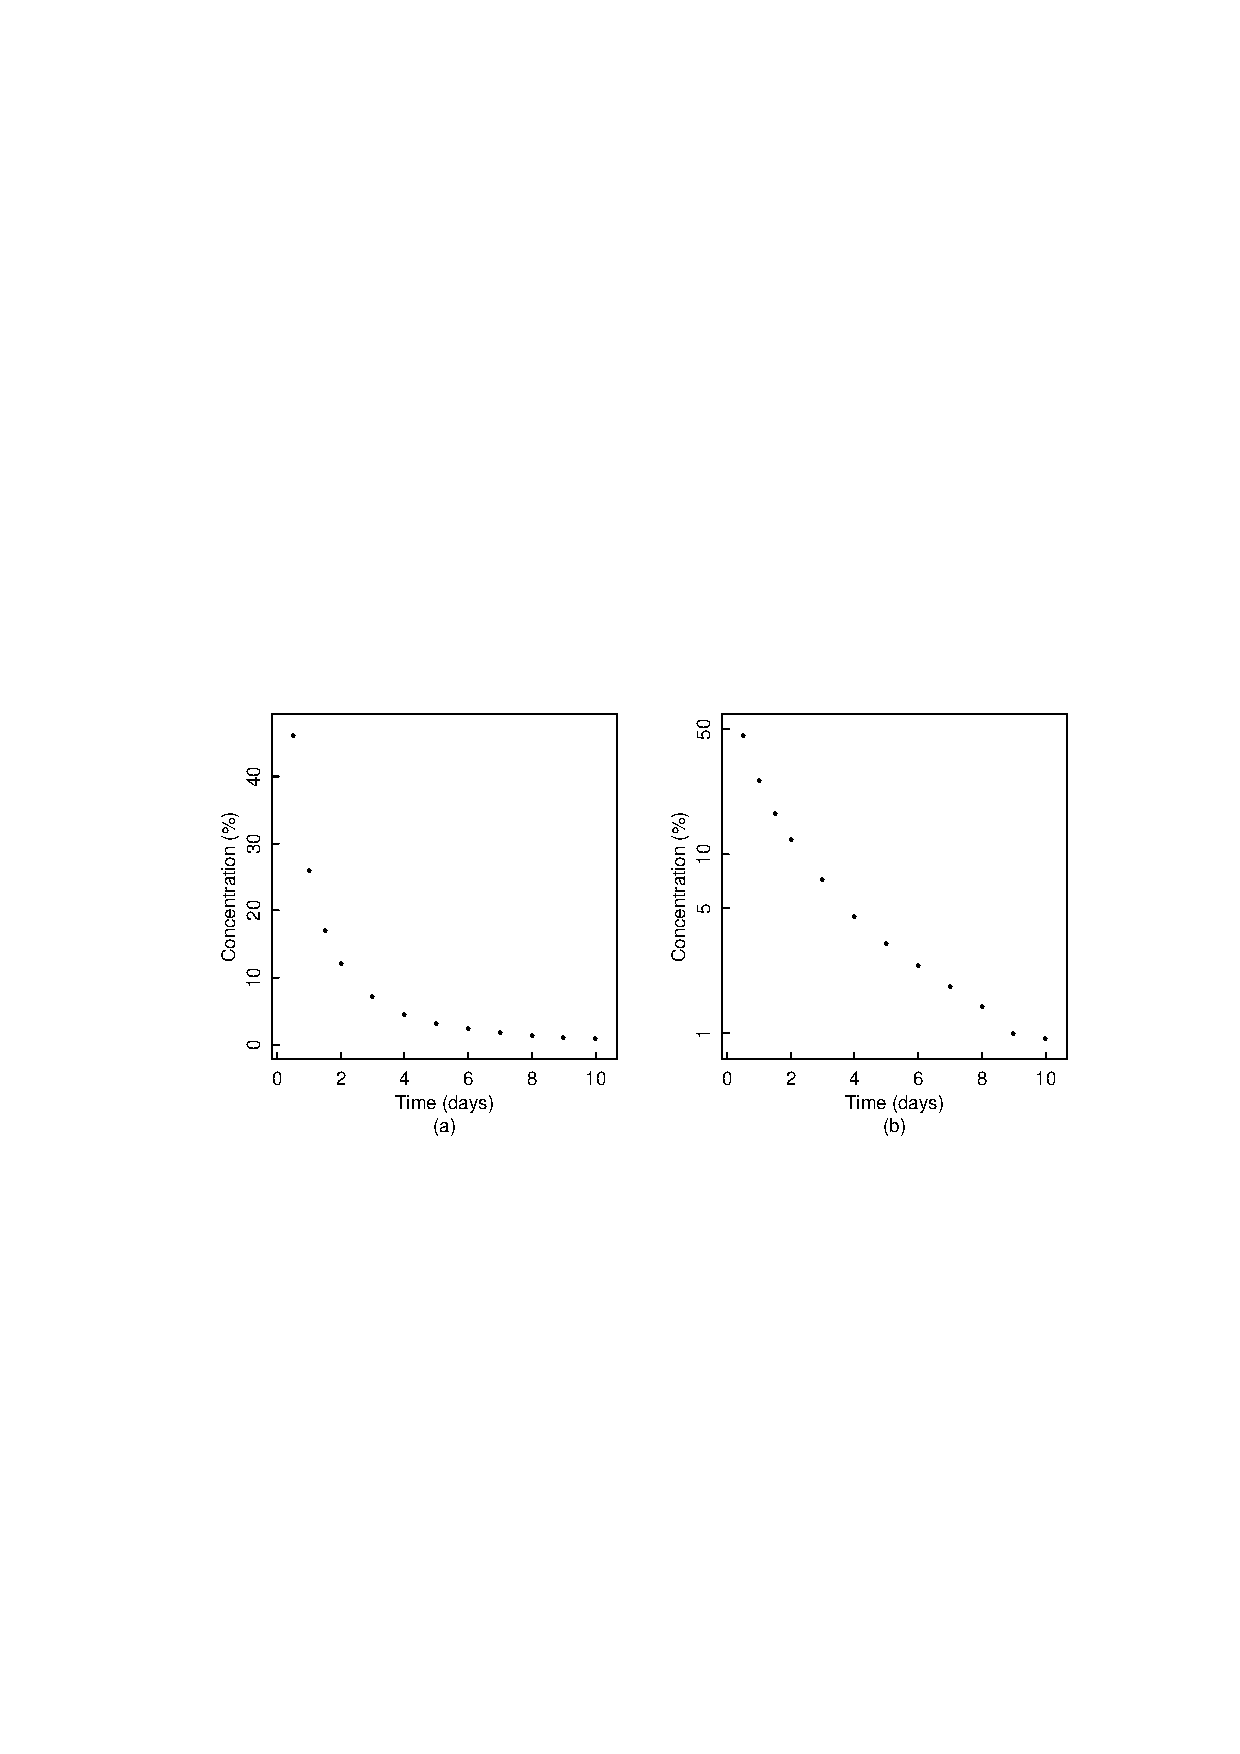
\includegraphics{5LIPdata}}%,height=3in}}
  \caption{\label{fig:LIPdata}
  Plot of the lipoprotein concentration versus time, on a linear scale
  in part $a$, and on a logarithmic scale in part $b$.
  }
\end{figure}
from which it can be seen that
there is a decrease in concentration through time, indicating
elimination from the serum compartment.
From a semilog plot of concentration versus time, it is apparent
that there are at least 2 compartments, but
to begin developing a model we fit a 1-compartment
elimination model, as shown in Figure~\ref{fig:1compart}.
\expandafter\ifx\csname graph\endcsname\relax \csname newbox\endcsname\graph\fi
\expandafter\ifx\csname graphtemp\endcsname\relax \csname newdimen\endcsname\graphtemp\fi
\setbox\graph=\vtop{\vskip 0pt\hbox{%
    \special{pn 8}%
    \special{ar 250 250 250 250 0 6.28319}%
    \graphtemp=.5ex\advance\graphtemp by 0.250in
    \rlap{\kern 0.250in\lower\graphtemp\hbox to 0pt{\hss $\gamma_{1}$\hss}}%
    \special{pa 250 500}%
    \special{pa 250 1000}%
    \special{fp}%
    \special{sh 1.000}%
    \special{pa 275 900}%
    \special{pa 250 1000}%
    \special{pa 225 900}%
    \special{pa 275 900}%
    \special{fp}%
    \graphtemp=.5ex\advance\graphtemp by 0.750in
    \rlap{\kern 0.250in\lower\graphtemp\hbox to 0pt{\hss $\theta$ }}%
    \hbox{\vrule depth1.000in width0pt height 0pt}%
    \kern 0.500in
  }%
}%

\begin{figure}
  \centerline{\box\graph}
  \caption{\label{fig:1compart}
  A 1-compartment elimination model.
  }
\end{figure}

\subsection{One Compartment}

We see from the plot that the concentration has reached
46\% by time 0.5 day, and so the starting value for the
rate constant is
\begin{eqnarray*}
  \theta&=&{- \ln0.46 \over 0.5 }\\
  &\approx&1.55
\end{eqnarray*}

Convergence to $ \hat \theta = 1.31$ was achieved
with a residual sum of squares of 133 on 11 degrees of freedom.

\subsection{Two Compartments}

The residuals, plotted against time in Figure~\ref{fig:LIPres1}, have a
\begin{figure}
  \centerline{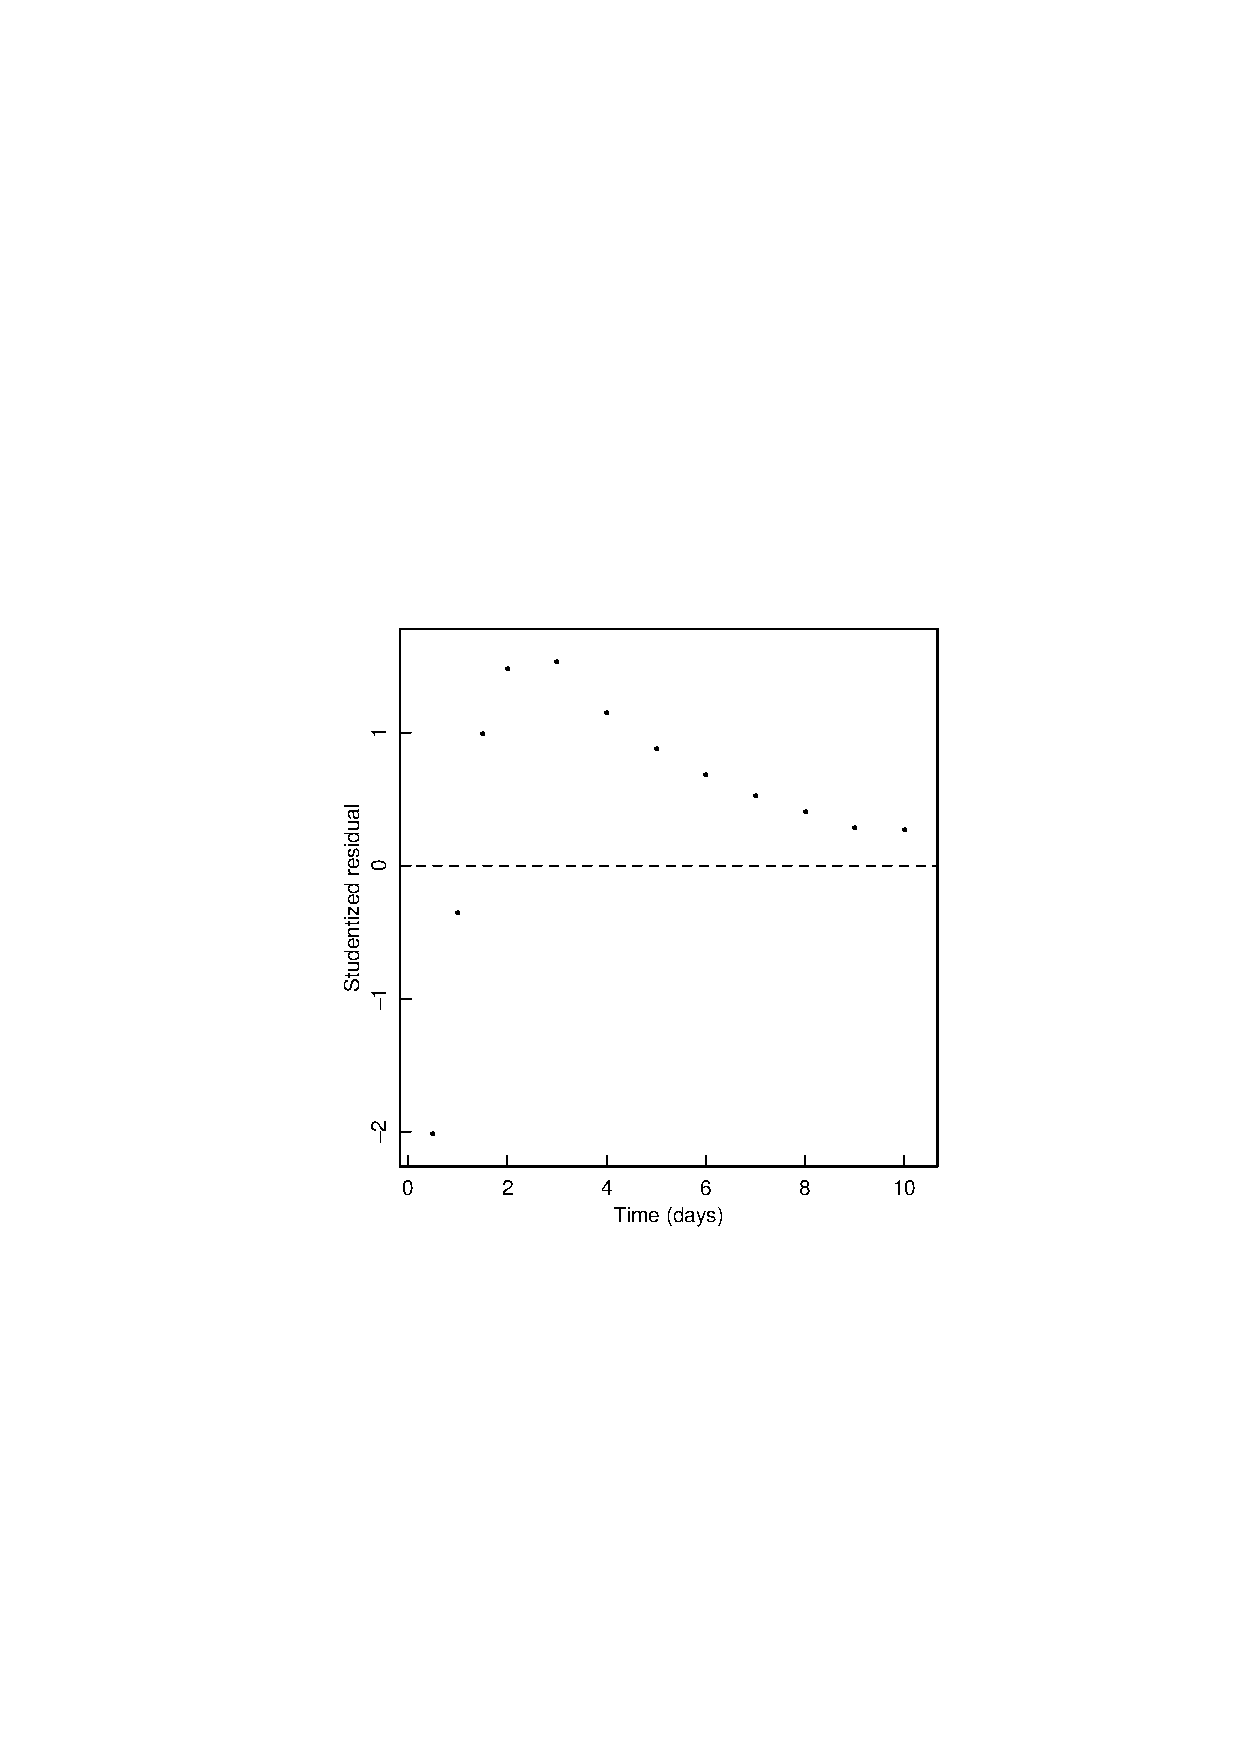
\includegraphics{5LIPres1}}%,height=4in}}
  \caption{\label{fig:LIPres1}
  Residuals from a 1-compartment model fitted to the lipoprotein data.
  }
\end{figure}
noticeable pattern, suggesting that the model initially
underestimates and then overestimates the concentration.
This pattern is consistent with the presence of
another compartment with a system diagram as in
Figure~\ref{fig:twocomp},
\expandafter\ifx\csname graph\endcsname\relax \csname newbox\endcsname\graph\fi
\expandafter\ifx\csname graphtemp\endcsname\relax \csname newdimen\endcsname\graphtemp\fi
\setbox\graph=\vtop{\vskip 0pt\hbox{%
    \special{pn 8}%
    \special{ar 250 250 250 250 0 6.28319}%
    \graphtemp=.5ex\advance\graphtemp by 0.250in
    \rlap{\kern 0.250in\lower\graphtemp\hbox to 0pt{\hss $\gamma_{1}$\hss}}%
    \special{ar 1250 250 250 250 0 6.28319}%
    \graphtemp=.5ex\advance\graphtemp by 0.250in
    \rlap{\kern 1.250in\lower\graphtemp\hbox to 0pt{\hss $\gamma_{2}$\hss}}%
    \special{pa 427 73}%
    \special{pa 1073 73}%
    \special{fp}%
    \special{sh 1.000}%
    \special{pa 973 48}%
    \special{pa 1073 73}%
    \special{pa 973 98}%
    \special{pa 973 48}%
    \special{fp}%
    \graphtemp=\baselineskip\multiply\graphtemp by -1\divide\graphtemp by 2
    \advance\graphtemp by .5ex\advance\graphtemp by 0.073in
    \rlap{\kern 0.750in\lower\graphtemp\hbox to 0pt{\hss $\theta_{2}$\hss}}%
    \special{pa 427 427}%
    \special{pa 1073 427}%
    \special{fp}%
    \special{sh 1.000}%
    \special{pa 527 452}%
    \special{pa 427 427}%
    \special{pa 527 402}%
    \special{pa 527 452}%
    \special{fp}%
    \graphtemp=\baselineskip\multiply\graphtemp by -1\divide\graphtemp by 2
    \advance\graphtemp by .5ex\advance\graphtemp by 0.427in
    \rlap{\kern 0.750in\lower\graphtemp\hbox to 0pt{\hss $\theta_{3}$\hss}}%
    \special{pa 250 500}%
    \special{pa 250 1000}%
    \special{fp}%
    \special{sh 1.000}%
    \special{pa 275 900}%
    \special{pa 250 1000}%
    \special{pa 225 900}%
    \special{pa 275 900}%
    \special{fp}%
    \graphtemp=.5ex\advance\graphtemp by 0.750in
    \rlap{\kern 0.250in\lower\graphtemp\hbox to 0pt{\hss $\theta_{1}$ }}%
    \hbox{\vrule depth1.000in width0pt height 0pt}%
    \kern 1.500in
  }%
}%

\begin{figure}
  \centerline{\box\graph}
  \caption{\label{fig:twocomp}
  A 2-compartment open model.
  }
\end{figure}
possibly with $\theta_{2}$ and $\theta_{3}$ equal.
It is easy to fit such a 2-parameter model first and use the
estimates to provide starting values for a 3-parameter model.

To get starting estimates for the 2-parameter model, we let
$\theta_1 + \theta_2 = 1.31$ from the 1-compartment
model fit, and try $ \btheta^0 = ( 1.0,  0.31 ) \trans$.
Convergence was obtained to
$\hat \btheta = ( 0.992 ,  0.663) \trans$ with a
residual sum of squares of 2.65 on 10 degrees of freedom.
Allowing $\theta_{2}$ and $\theta_{3}$ to differ,
we used starting estimates
$\btheta^0=(0.99,0.67,0.65)\trans $, which yielded
$\hat\btheta=(1.022,0.662,0.820)\trans$ with a residual sum of
squares of 1.26 on 9 degrees of freedom.

\subsection{Three Compartments}

The residuals from the 3-parameter model, plotted in
Figure~\ref{fig:LIPres2c3p},
\begin{figure}
  \centerline{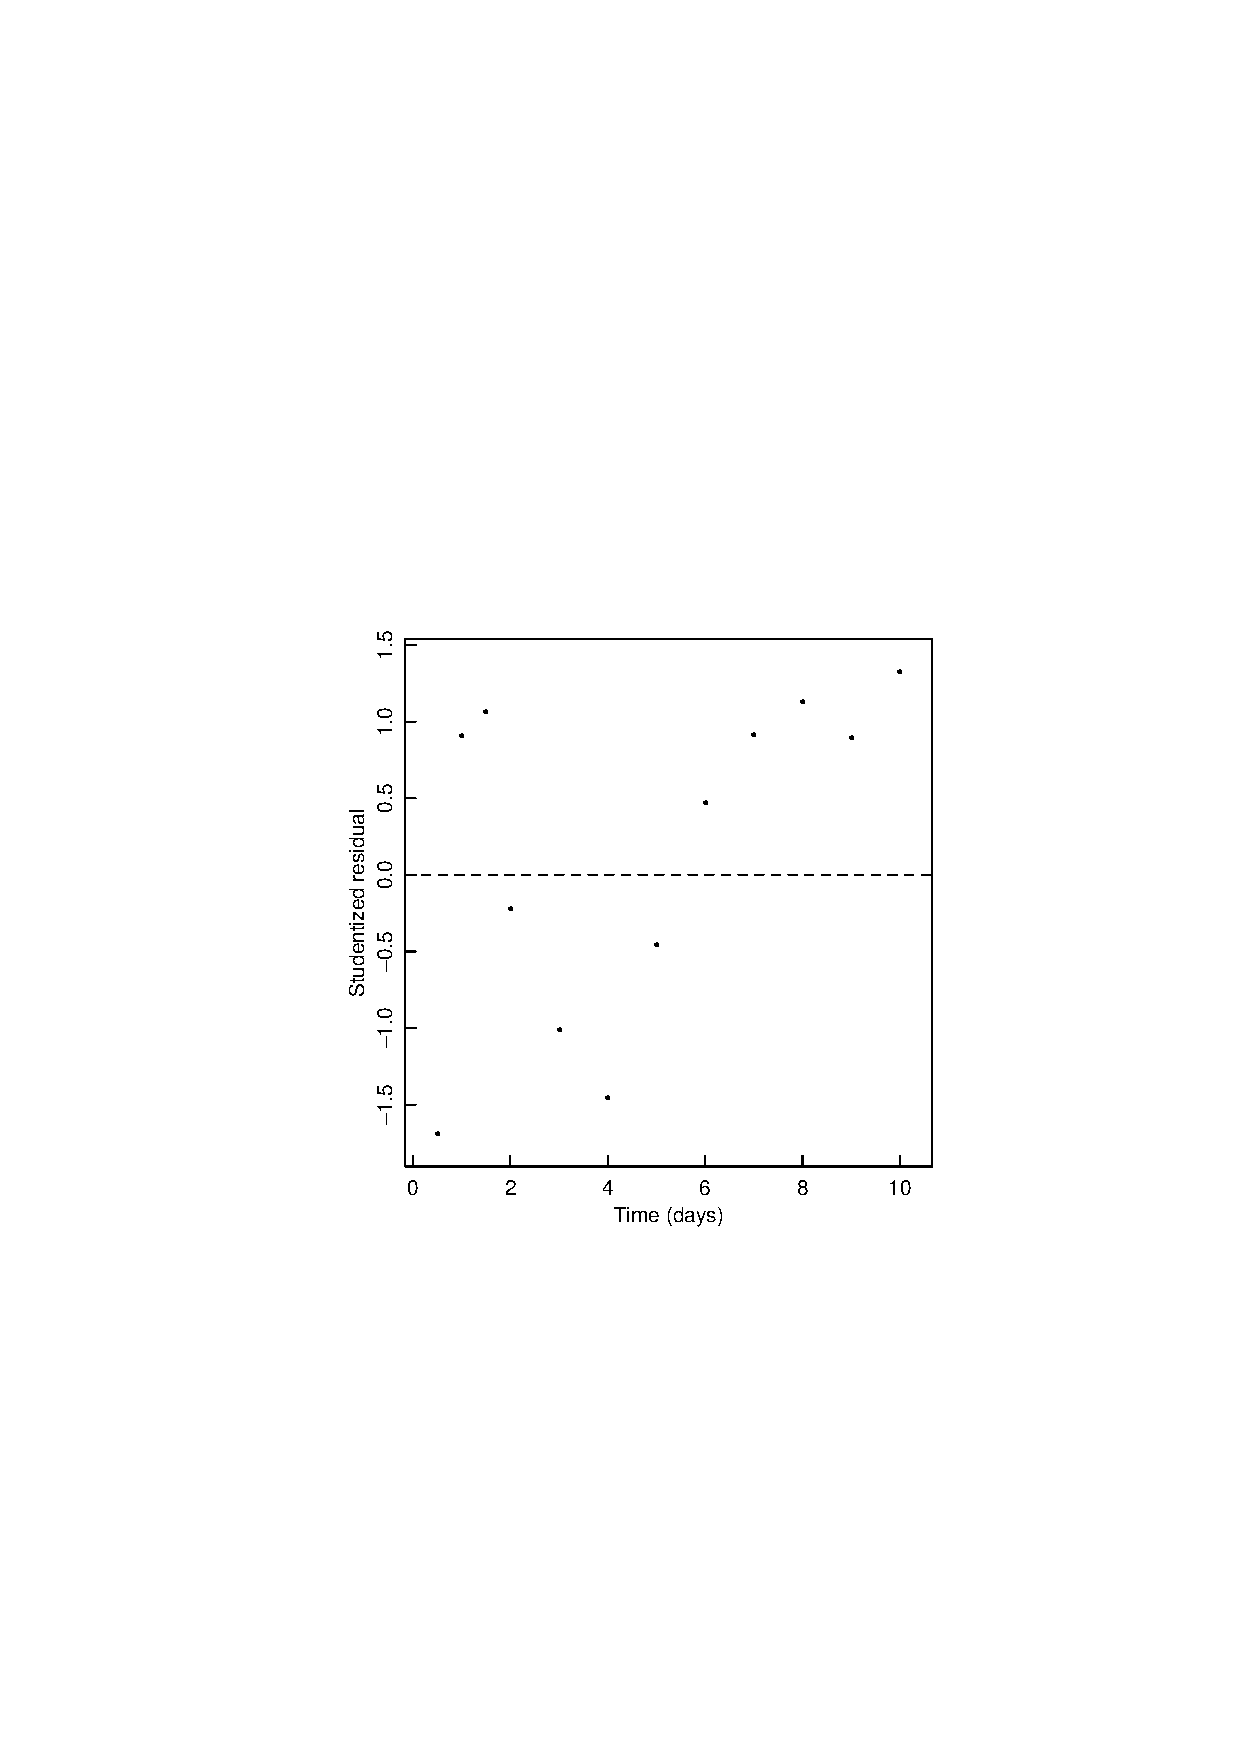
\includegraphics{5LIPres2c3p}}%,height=4in}}
  \caption{\label{fig:LIPres2c3p}
  Residuals from a 2-compartment model fitted to the lipoprotein data.
  }
\end{figure}
still display a pattern, so we continue to extend the model.
We can extend it in a number of different ways:
if the experimenter was uncertain how the concentrations
were normalized to produce $ \gamma_1 ( 0 ) = 100$,
we could introduce a parameter to represent this
initial value, or we could introduce a delay time into the model,
or (as seems more appropriate in this case) we could introduce
another compartment.
Even when introducing a third compartment, however, we must
decide how to do so.
The simplest extensions are the {\em catenary\/}
system (in which the compartments are chained together),
\index{compartment model!catenary}
and the {\em mamillary\/} system (in which each
``daughter'' compartment communicates only with the central
``mother'' compartment.)
\index{compartment model!mamillary}
A catenary system is shown in
Figure~\ref{fig:catenary},
\expandafter\ifx\csname graph\endcsname\relax \csname newbox\endcsname\graph\fi
\expandafter\ifx\csname graphtemp\endcsname\relax \csname newdimen\endcsname\graphtemp\fi
\setbox\graph=\vtop{\vskip 0pt\hbox{%
    \special{pn 8}%
    \special{ar 250 250 250 250 0 6.28319}%
    \graphtemp=.5ex\advance\graphtemp by 0.250in
    \rlap{\kern 0.250in\lower\graphtemp\hbox to 0pt{\hss $\gamma_{1}$\hss}}%
    \special{ar 1250 250 250 250 0 6.28319}%
    \graphtemp=.5ex\advance\graphtemp by 0.250in
    \rlap{\kern 1.250in\lower\graphtemp\hbox to 0pt{\hss $\gamma_{2}$\hss}}%
    \special{ar 2250 250 250 250 0 6.28319}%
    \graphtemp=.5ex\advance\graphtemp by 0.250in
    \rlap{\kern 2.250in\lower\graphtemp\hbox to 0pt{\hss $\gamma_{3}$\hss}}%
    \special{pa 250 500}%
    \special{pa 250 1000}%
    \special{fp}%
    \special{sh 1.000}%
    \special{pa 275 900}%
    \special{pa 250 1000}%
    \special{pa 225 900}%
    \special{pa 275 900}%
    \special{fp}%
    \graphtemp=.5ex\advance\graphtemp by 0.750in
    \rlap{\kern 0.250in\lower\graphtemp\hbox to 0pt{\hss $\theta_{1}$ }}%
    \special{pa 427 73}%
    \special{pa 1073 73}%
    \special{fp}%
    \special{sh 1.000}%
    \special{pa 973 48}%
    \special{pa 1073 73}%
    \special{pa 973 98}%
    \special{pa 973 48}%
    \special{fp}%
    \graphtemp=\baselineskip\multiply\graphtemp by -1\divide\graphtemp by 2
    \advance\graphtemp by .5ex\advance\graphtemp by 0.073in
    \rlap{\kern 0.750in\lower\graphtemp\hbox to 0pt{\hss $\theta_{2}$\hss}}%
    \special{pa 427 427}%
    \special{pa 1073 427}%
    \special{fp}%
    \special{sh 1.000}%
    \special{pa 527 452}%
    \special{pa 427 427}%
    \special{pa 527 402}%
    \special{pa 527 452}%
    \special{fp}%
    \graphtemp=\baselineskip\multiply\graphtemp by -1\divide\graphtemp by 2
    \advance\graphtemp by .5ex\advance\graphtemp by 0.427in
    \rlap{\kern 0.750in\lower\graphtemp\hbox to 0pt{\hss $\theta_{3}$\hss}}%
    \special{pa 1427 73}%
    \special{pa 2073 73}%
    \special{fp}%
    \special{sh 1.000}%
    \special{pa 1973 48}%
    \special{pa 2073 73}%
    \special{pa 1973 98}%
    \special{pa 1973 48}%
    \special{fp}%
    \graphtemp=\baselineskip\multiply\graphtemp by -1\divide\graphtemp by 2
    \advance\graphtemp by .5ex\advance\graphtemp by 0.073in
    \rlap{\kern 1.750in\lower\graphtemp\hbox to 0pt{\hss $\theta_{4}$\hss}}%
    \special{pa 1427 427}%
    \special{pa 2073 427}%
    \special{fp}%
    \special{sh 1.000}%
    \special{pa 1527 452}%
    \special{pa 1427 427}%
    \special{pa 1527 402}%
    \special{pa 1527 452}%
    \special{fp}%
    \graphtemp=\baselineskip\multiply\graphtemp by -1\divide\graphtemp by 2
    \advance\graphtemp by .5ex\advance\graphtemp by 0.427in
    \rlap{\kern 1.750in\lower\graphtemp\hbox to 0pt{\hss $\theta_{5}$\hss}}%
    \hbox{\vrule depth1.000in width0pt height 0pt}%
    \kern 2.500in
  }%
}%

\begin{figure}
  \centerline{\box\graph}
  \caption{\label{fig:catenary}
  A 3-compartment catenary model.  }
\end{figure}
and a mamillary system is shown in Figure~\ref{fig:mamillary}.
\expandafter\ifx\csname graph\endcsname\relax \csname newbox\endcsname\graph\fi
\expandafter\ifx\csname graphtemp\endcsname\relax \csname newdimen\endcsname\graphtemp\fi
\setbox\graph=\vtop{\vskip 0pt\hbox{%
    \special{pn 8}%
    \special{ar 250 1000 250 250 0 6.28319}%
    \graphtemp=.5ex\advance\graphtemp by 1.000in
    \rlap{\kern 0.250in\lower\graphtemp\hbox to 0pt{\hss $\gamma_{1}$\hss}}%
    \special{ar 1250 1000 250 250 0 6.28319}%
    \graphtemp=.5ex\advance\graphtemp by 1.000in
    \rlap{\kern 1.250in\lower\graphtemp\hbox to 0pt{\hss $\gamma_{3}$\hss}}%
    \special{ar 250 250 250 250 0 6.28319}%
    \graphtemp=.5ex\advance\graphtemp by 0.250in
    \rlap{\kern 0.250in\lower\graphtemp\hbox to 0pt{\hss $\gamma_{2}$\hss}}%
    \special{pa 250 1250}%
    \special{pa 250 1750}%
    \special{fp}%
    \special{sh 1.000}%
    \special{pa 275 1650}%
    \special{pa 250 1750}%
    \special{pa 225 1650}%
    \special{pa 275 1650}%
    \special{fp}%
    \graphtemp=.5ex\advance\graphtemp by 1.500in
    \rlap{\kern 0.250in\lower\graphtemp\hbox to 0pt{\hss $\theta_{1}$ }}%
    \special{pa 73 823}%
    \special{pa 73 427}%
    \special{fp}%
    \special{sh 1.000}%
    \special{pa 48 527}%
    \special{pa 73 427}%
    \special{pa 98 527}%
    \special{pa 48 527}%
    \special{fp}%
    \graphtemp=.5ex\advance\graphtemp by 0.625in
    \rlap{\kern 0.073in\lower\graphtemp\hbox to 0pt{\hss $\theta_{2}$ }}%
    \special{pa 427 823}%
    \special{pa 427 427}%
    \special{fp}%
    \special{sh 1.000}%
    \special{pa 452 723}%
    \special{pa 427 823}%
    \special{pa 402 723}%
    \special{pa 452 723}%
    \special{fp}%
    \graphtemp=.5ex\advance\graphtemp by 0.625in
    \rlap{\kern 0.427in\lower\graphtemp\hbox to 0pt{\hss $\theta_{3}$ }}%
    \special{pa 427 823}%
    \special{pa 1073 823}%
    \special{fp}%
    \special{sh 1.000}%
    \special{pa 973 798}%
    \special{pa 1073 823}%
    \special{pa 973 848}%
    \special{pa 973 798}%
    \special{fp}%
    \graphtemp=\baselineskip\multiply\graphtemp by -1\divide\graphtemp by 2
    \advance\graphtemp by .5ex\advance\graphtemp by 0.823in
    \rlap{\kern 0.750in\lower\graphtemp\hbox to 0pt{\hss $\theta_{4}$\hss}}%
    \special{pa 427 1177}%
    \special{pa 1073 1177}%
    \special{fp}%
    \special{sh 1.000}%
    \special{pa 527 1202}%
    \special{pa 427 1177}%
    \special{pa 527 1152}%
    \special{pa 527 1202}%
    \special{fp}%
    \graphtemp=\baselineskip\multiply\graphtemp by -1\divide\graphtemp by 2
    \advance\graphtemp by .5ex\advance\graphtemp by 1.177in
    \rlap{\kern 0.750in\lower\graphtemp\hbox to 0pt{\hss $\theta_{5}$\hss}}%
    \hbox{\vrule depth1.750in width0pt height 0pt}%
    \kern 1.500in
  }%
}%

\begin{figure}
  \centerline{\box\graph}
  \caption{\label{fig:mamillary}
  A 3-compartment mamillary model.  }
\end{figure}

To fit these systems, we could use 5, 4, or 3 parameters by
assuming some of the parameters equal.
We chose to fit the 5-parameter models and examine the fits to
determine a simple adequate model.

For the catenary model we added two parameters with values smaller
than, and distinct from,
the current parameter estimates to produce the starting estimates
$$
\btheta^0 = ( 1.00 ,  0.66 ,  0.82 ,  0.5 ,  0.2 ) \trans
$$
from which we converged to
$$
\hat \btheta = ( 0.990 ,  0.762 ,  1.015 ,  0.240 ,  0.352 ) \trans
$$
with a residual sum of squares of 0.043 on 7 degrees of freedom.

Using the same starting values, the mamillary model converged to
$$
\hat \btheta = ( 0.990 ,  0.532 ,  1.340 ,  0.231 ,  0.267 ) \trans
$$
with the same residual sum of squares as the catenary model.
The residuals (for both models) are shown in
Figure~\ref{fig:LIPres3cm5p},
\begin{figure}
  \centerline{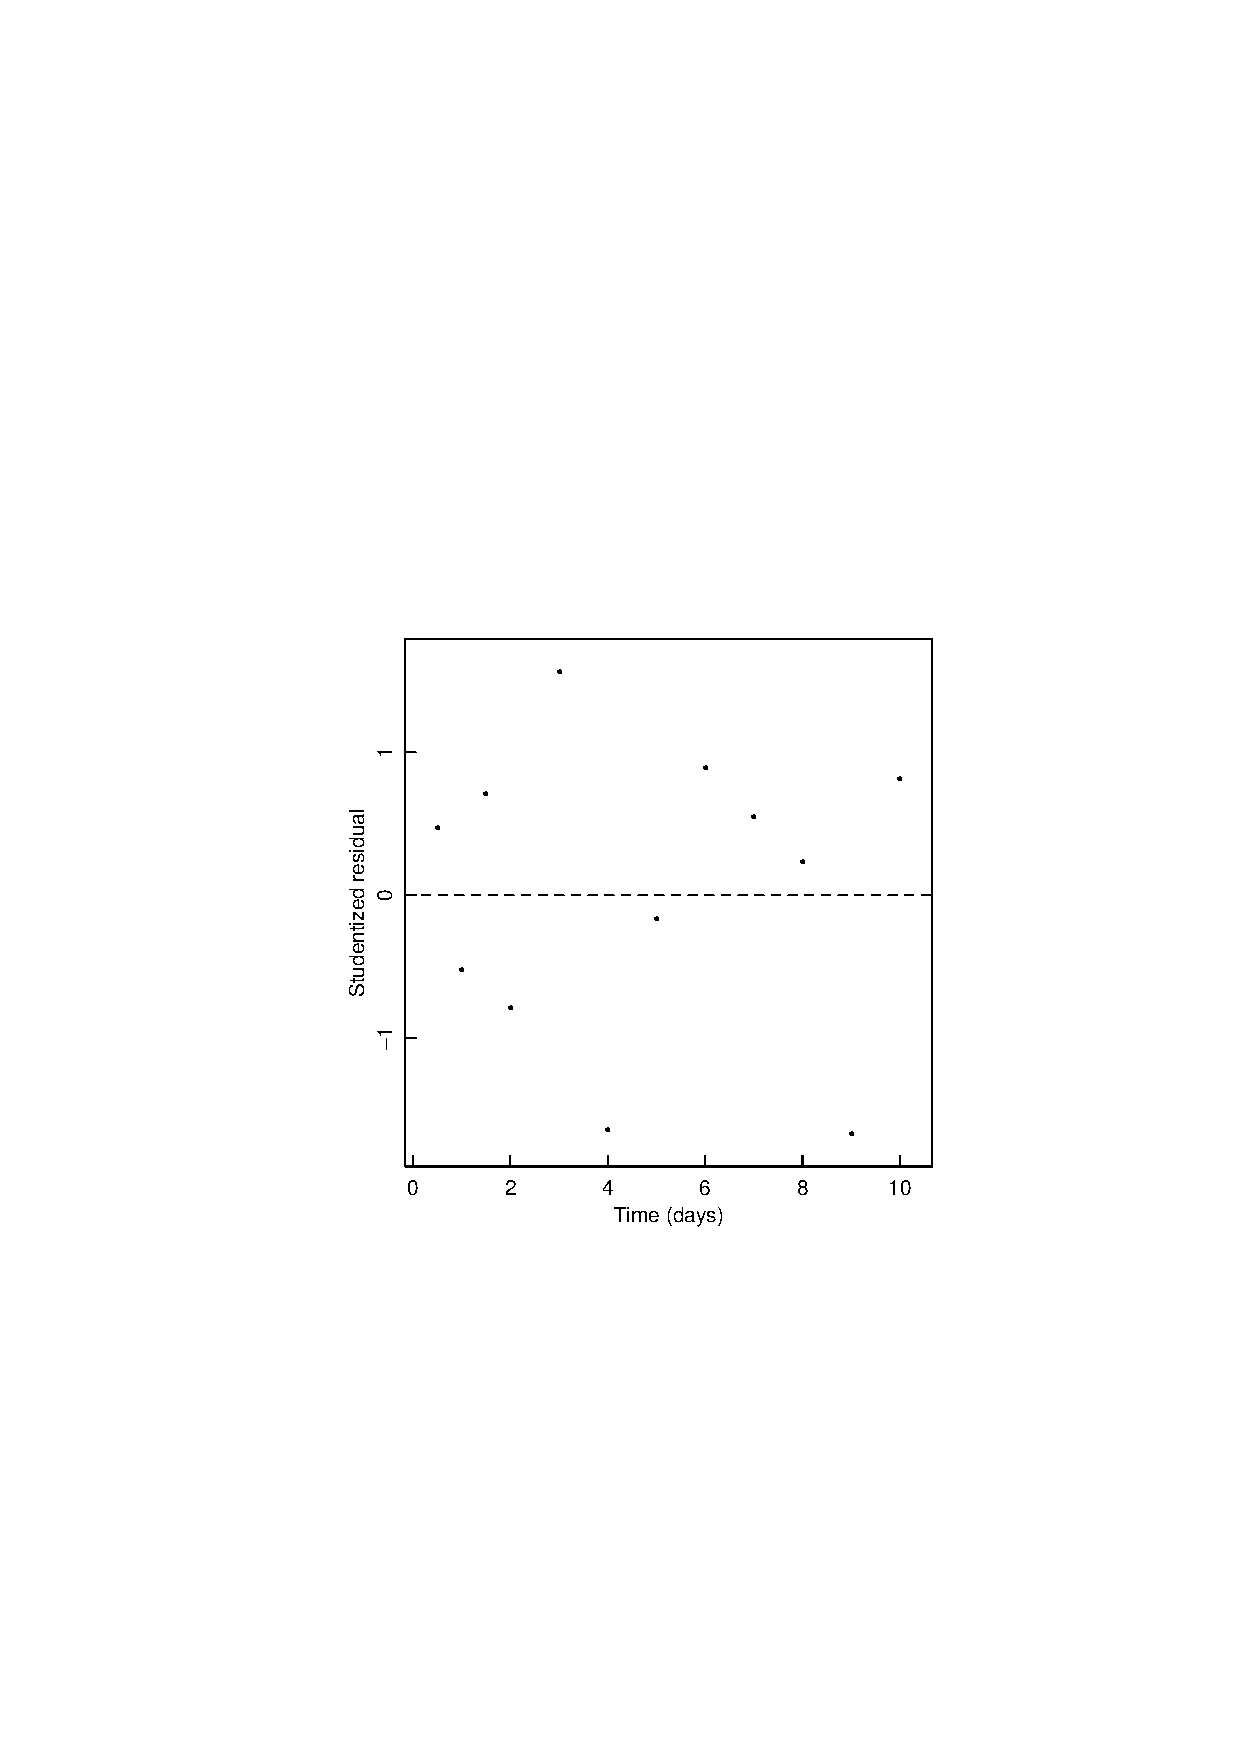
\includegraphics{5LIPres3cm5p}}%,height=4in}}
  \caption{\label{fig:LIPres3cm5p}
  Residuals from a 3-compartment model fitted to the lipoprotein data.
  }
\end{figure}
and are well behaved.

It is not an accident that
the same residuals and the same sum of squares occur for these two
models, since they are equivalent when compartment 1 is the only
one measured.
Thus, for this data set, the model is not identifiable.
Writing $\bphi$ for the parameters of the catenary model and
$\btheta$ for the mamillary model parameters, the equivalence is
given by
\begin{eqnarray*}
  \phi_1&=&\theta_1\\
  \phi_2&=&\theta_2 + \theta_4\\
  \phi_3 + \phi_4 + \phi_5&=&\theta_3 + \theta_5\\
  \phi_3 \phi_5&=&\theta_3 \theta_5\\
  \phi_2 \phi_4 + \phi_2 \phi_5&=&\theta_2 \theta_5 + \theta_3 \theta_4
\end{eqnarray*}

\subsection{Three Compartments, Common Parameters}

The extra sum of squares due to extending the model from two to three
compartments was highly significant [an extra sum of squares ratio of 97
to be compared with an $F ( 2, 7 ) $ distribution].
We now try to simplify the model by
letting some parameters be equal.
We take starting values from the 5-parameter fits using the
average of the pair of rate constants with the smallest
difference relative to the standard error of the difference,
so that, for both models, we equate $ \theta_{4}$ and $ \theta_{5}$.
For the catenary model, we converged to
$\hat \btheta = ( 0.967 ,  0.778 ,  0.948 ,  0.224 ) \trans$ with a
residual sum of squares of 0.062, and for
the mamillary model, to
$ \hat \btheta = ( 0.978 ,  0.558 ,  1.27 ,  0.213 ) \trans$
with a residual sum of squares of 0.050.
The parameter estimates and approximate standard errors strongly
suggest that none of the other parameters are equal, and so
we do not reduce the models further.

Normal plots and plots of the residuals versus time and versus the
fitted response (not shown) did not show inadequacy of the 4-parameter
models.
The judgement of which model to use must then be based on extra sum of
squares analyses and the opinion of the experimenter as to which model
is better.
Extra sum of squares analyses for the nested models are shown
in Table~\ref{tbl:5.3}.
\begin{table}
  \begin{tabular}{l r r r r r}
    %c c c c c c
    %c c c c c c
    %l c c c c c
    %l n n n n n.
    %\_
    %:Sum of:Degrees:Mean
    %:Squares:of:Square
    %Source:$(10^{-6} )$:Freedom:$(10^{-7} )$:F Ratio:$p$ Value
    %\par\vspace{2.0pt}
    %\_
    %Extra:1.857:1:18.57:3.0:0.13
    %Model 3:4.339:7:6.20
    %\par\vspace{6.0pt}
    %Model 1:6.196:8
    %\_
    %Extra:0.682:1:6.82:1.1:0.33
    %Model 3:4.339:7:6.20
    %\par\vspace{6.0pt}
    %Model 2:5.021:8
    %\_
  \end{tabular}
  \caption{\label{tbl:5.3}
  Extra sum of squares analyses for compartment models fitted to the
  lipoprotein data.
  The models with 4 parameters are the 3-compartment catenary (model 1)
  and the 3-compartment mamillary (model 2), each with two of the rate
  constants contrained to be equal.
  The 5-parameter 3-compartment model is model 3.
  }
\end{table}

\subsection{Conclusions}

The conclusion of this analysis is that the data can be
adequately fitted by a 3-compartment model in either the catenary
or mamillary configuration.
For five rate constants, the two models are equivalent:
for four rate constants, slightly better results are obtained
with the mamillary configuration.
Whether or not equal rate constants is physically sensible must
be decided by the experimenter on the basis of theory or on the
basis of further experimental results.

\section{Oil Shale: A Case Study}

As an example of multiresponse parameter estimation
\index{multiresponse estimation!compartment model}
\index{compartment model!multiresponse estimation}
using compartment models, we return to the oil shale data obtained by
\citeasnoun{hubb:robi:1950}.
%\glossary{ Hubbard, A.B.}
%\glossary{ Robinson, W.E.}
This case study also demonstrates the use of process
parameters to model kinetic parameters (see Section 3.11).
\index{parameter!process}
\index{parameter!kinetic}
\subsection{Preliminary Analysis}

In Figure~\ref{fig:OILdata}
\begin{figure}
  \centerline{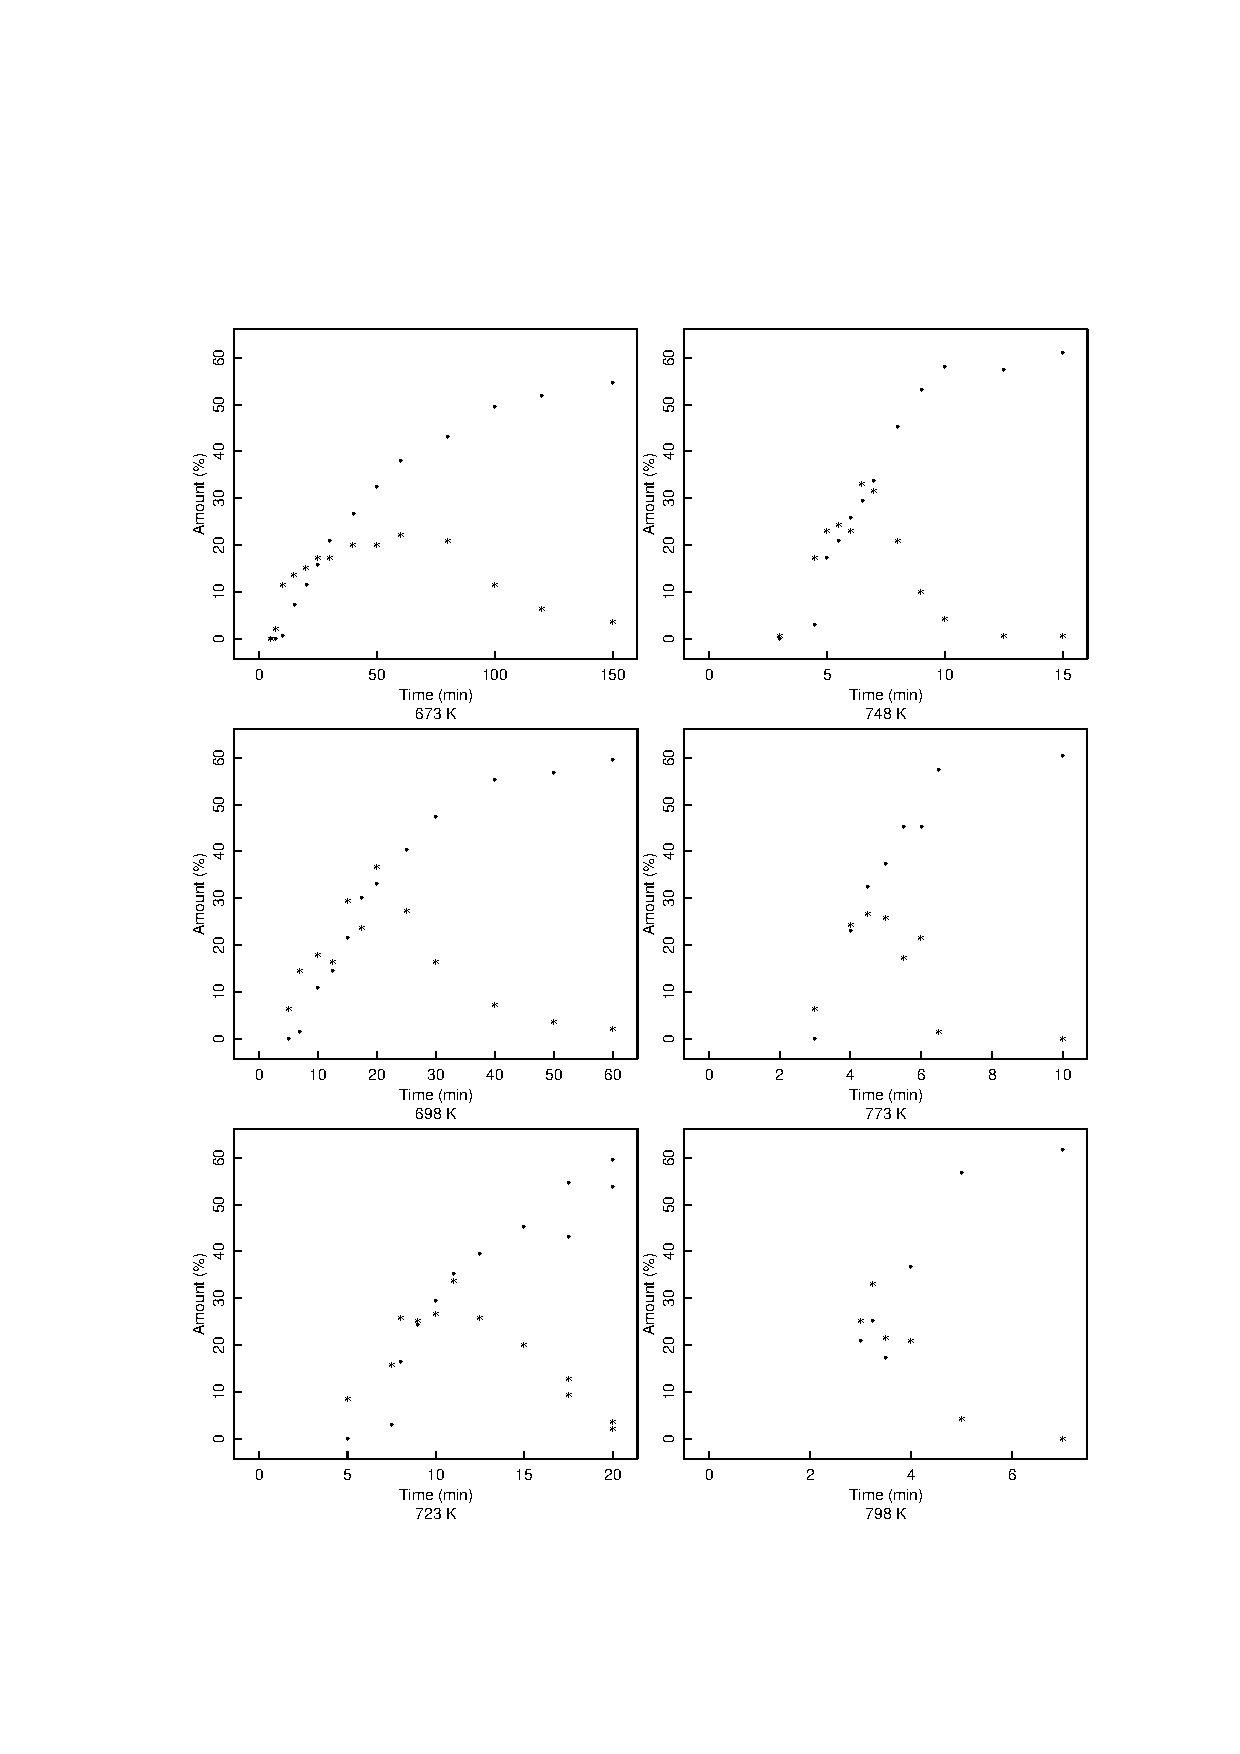
\includegraphics{5OILdata}}%,width=\textwidth}}
  \caption{\label{fig:OILdata}
  Plot of oil ($\bullet$) and bitumen ($*$) amounts versus time
  for six temperatures for the oil shale pyrolysis data.
  }
\end{figure}
we plot the two measured responses, oil and bitumen, versus time
for the six temperatures.
One thing to note from these plots is that kerogen decomposition
occurs more rapidly with increased temperature;
at 673K there is a substantial fraction
of bitumen after 100 minutes, but at 773K there
is only a small fraction after 10 minutes.
This strongly suggests that the rate constants depend on temperature.

A common form of rate constant dependence upon temperature
is the Arrhenius relation
\index{Arrhennius relation}
$$\label{eqn:arrhen}
{\rm k}_i ( T ) = {\rm k}_{i,0} 
e^{{-} E_i / R T}
$$
where $\mbox{\rm k}_i ( T )$ is the rate constant at temperature $T$,
$\mbox{\rm k}_{i,0}$ is the preexponential term, $E_{i}$ is the activation
energy for the reaction, $R$ is the universal gas constant of 1.987
cal/g-moleK, and $T$ is the temperature in kelvins.

Estimating the activation energies and the preexponential
terms usually results in highly correlated estimates, since
the range of the observed temperatures is small
relative to the mean temperature.
To reduce the correlations, we center the temperatures about
an intermediate temperature, $T_{0}$, as discussed in Section 3.4.2,
and write (\ref{eqn:arrhen})
as
$$
{\rm k}_i ( T ) = {\rm k}_i ( T_0 ) 
\exp {\left[ - { E_i   \over R }\left( {1 \over T }-
{1 \over T_0} \right)\right]}
$$
Then
\begin{eqnarray}\label{eqn:logarr}
  \ln{\rm k}_i ( T )&=&\ln{\rm k}_i ( T_0 )
  - {E_i  \over R }\left( {1 \over T }- {1 \over T_0}\right)\\
  &=&\phi_i
  - {E_i  \over R }\left( {1 \over T }- {1 \over T_0}\right)\nonumber
\end{eqnarray}
so the logarithms of the rate constants depend linearly
on the scaled inverse temperature.

\subsection{Starting Values for the 673K Data}

To determine starting values for the process parameters, we first fit
the kinetic model to the data at each individual temperature.  This
means that we must find starting estimates for the kinetic parameters,
which can be done by modifying the approximate rate method described
in Section 4.3.1.

For these data sets, only
bitumen and oil have been measured at each time.
The kerogen percentage is not measured,
nor can it be inferred from a mass balance, since the
by-products, coke and gas, are not measured either.
However, we know that at time 0 the kerogen percentage is 100
while the percentage of the other species is zero.
Substituting these values into the model
\begin{eqnarray*}
  { d \gamma_1   \over  d t }&=&- ( \theta_1 + \theta_4 ) \gamma_1\\
  {d\gamma_2\over d t }&=&\theta_1 \gamma_1 -
  ( \theta_2 + \theta_3 ) \gamma_2\\
  { d \gamma_3   \over  d t }&=&\theta_4 \gamma_1 + \theta_2 \gamma_2
\end{eqnarray*}
at time 0 produces
\begin{eqnarray*}
  {d \gamma_2 ( 0 )  \over d t}&=&\theta_1\gamma_1 ( 0 )\\
  &=& 100  \theta_1
\end{eqnarray*}
and
$$
{d \gamma_3 ( 0 )  \over d t} = 100  \theta_4
$$
and we can use approximate rates from early observations of
$\gamma_{2}$ and $\gamma_{3}$ to obtain starting estimates
$\theta_1^{0}$ and $\theta_4^{0}$.
From these, we can infer a percentage of kerogen as
$$
\gamma_1 ( t )  \approx 
100  e^{ - ( \theta_1^0 + \theta_4^0 ) t }
$$
and use the approximate rate method of Section 4.3.1 to obtain
starting estimates $\theta_2^{0}$ and $\theta_3^{0}$.

The plot of the 673K data in Figure~\ref{fig:OILdata}
reveals evidence of dead time in the reactions, as described in
\index{dead time}
\citeasnoun{zieg:gorm:1980}.
%\glossary{ Ziegel, E.R.}
%\glossary{ Gorman, J.W.}
We therefore use the first two nonzero observations of $\gamma_{2}$
and $\gamma_{3}$ to calculate $\theta_1^{0}$ and
$\theta_4^{0}$ as
\begin{eqnarray*}
  \theta_1^0&=&\left. {1 \over \gamma_1 ( 0 )} 
  {d \gamma_2  \over d t} \right|_0\\
  &=& {1 \over 100 } {11.5 - 2.2  \over 3 }\\
  &=& 0.031
\end{eqnarray*}
and
\begin{eqnarray*}
  \theta_4^0&=& {1 \over 100 } {7.2 - 0.7  \over 5 }\\
  &=&  0.013  
\end{eqnarray*}
A starting estimate of the dead time, $t_0^0 = 6$ minutes, is
read from Figure~\ref{fig:OILdata}.
Using these values in the approximate rate procedure produces
starting estimates of 0.0131 for $\theta_2^{0}$ and 0.0286
for $\theta_3^{0}$.

\subsection{Fitting the Individual Temperature Data}

The generalized Gauss--Newton algorithm converged to the parameter
estimates shown in Table~\ref{tbl:oil.400}
\begin{table}
  \caption{\label{tbl:oil.400}
  Parameter summary for the oil shale data at 673K.
  }
  \begin{tabular}{l r r r r r}
    \mbox{}
    %c c c s s s s s s
    %c c c s s s s s s
    %c c c c c s s s s
    %c c c c c s s s s
    %c n n n n 1 n 1 n 1 n 1 n.
    %\_
    %::Logarithm Scale
    %\par\vspace{2.0pt}
    %::
    %:::Std.:Correlation
    %Parameter:Value:$ln\theta $:Error:Matrix
    %\par\vspace{2.0pt}
    %\_
    %$\theta_{1}$:0.0172:--4.064:0.1219:1.00
    %$\theta_{2}$:0.00891:--4.721:0.2524:0.85:1.00
    %$\theta_{3}$:0.0200:--3.912:0.1117:0.30:0.64:1.00
    %$\theta_{4}$:0.0105:--4.557:0.0645:--\/0.71:--\/0.89:--\/0.36:1.00
    %$t_{0}$:7.772::0.5263:--\/0.07:--\/0.34:--\/0.09:0.64:1.00
    %\par\vspace{4.0pt}
    %\_
  \end{tabular}
\end{table}
with a determinant value of 428.

The converged values for the 673K data can be used as
starting estimates for the 698K data, except for the dead time
which we estimate from Figure~\ref{fig:OILdata} to be 5 minutes.
Convergence was obtained to the results shown
in Table~\ref{tbl:oil.425}.
\begin{table}
  \caption{\label{tbl:oil.425}
  Parameter summary for the oil shale data at 698K.
  }
  \begin{tabular}{l r r r r r}
    %c c c s s s s s s
    %c c c s s s s s s
    %c c c c c s s s s
    %c c c c c s s s s
    %c n n n n 1 n 1 n 1 n 1 n.
    %\_
    %::Logarithm Scale
    %\par\vspace{2.0pt}
    %::
    %:::Std.:Correlation
    %Parameter:Value:$\ln\theta $:Error:Matrix
    %\_
    %$\theta_{1}$:0.0784:--2.546:0.1648:1.00
    %$\theta_{2}$:0.0473:--3.051:0.2270:0.46:1.00
    %$\theta_{3}$:0.0510:--2.975:0.1560:0.02:0.75:1.00
    %$\theta_{4}$:0.0249:--3.694:0.2290:--\/0.48:--\/0.91:--\/0.47:1.00
    %$t_{0}$:6.247::0.5065:--\/0.09:--\/0.53:--\/0.17:0.76:1.00
    %\_
  \end{tabular}
\end{table}

To obtain starting estimates for the kinetic parameters at the other
temperatures, we assume that an Arrhenius relation holds and
fit linear models to the logarithms of the rate constants
as a function of scaled inverse temperature.
Extrapolations of these linear fits are used to get starting
estimates for the kinetic parameters at the next temperature.
Since the dead time decreases with increasing temperature, we also
regress $t_{0}$ on scaled inverse temperature and extrapolate
to get starting estimates.

Care must be taken when fitting
the 723K data because there are two optima for the determinant
criterion, as shown in
Table~ \ref{tbl:450opt}.
\begin{table}
  \caption{\label{tbl:450opt}
  Parameter summary for the oil shale data at 723K, showing two optima.
  }
  \begin{tabular}{l r r r r r}
    %l 3 c 3 c
    %c l l.
    %\_
    %Parameter:Optimum 1:Optimum 2
    %\par\vspace{2.0pt}
    %\_
    %$\theta_{1}$:0.2637:0.1596
    %$\theta_{2}$:0.08496:0.1512
    %$\theta_{3}$:0.1587:0.1020
    %$\theta_{4}$:0.1248:0.02706
    %$t_{0}$:6.775:4.526
    %\par\vspace{4.0pt}
    %\_
    %Determinant:28309:53422
    %\par\vspace{2.0pt}
    %\_
  \end{tabular}
\end{table}
A plot of the data and the two sets of fitted curves, as in
Figure~\ref{fig:OIL450pred},
\begin{figure}
  \centerline{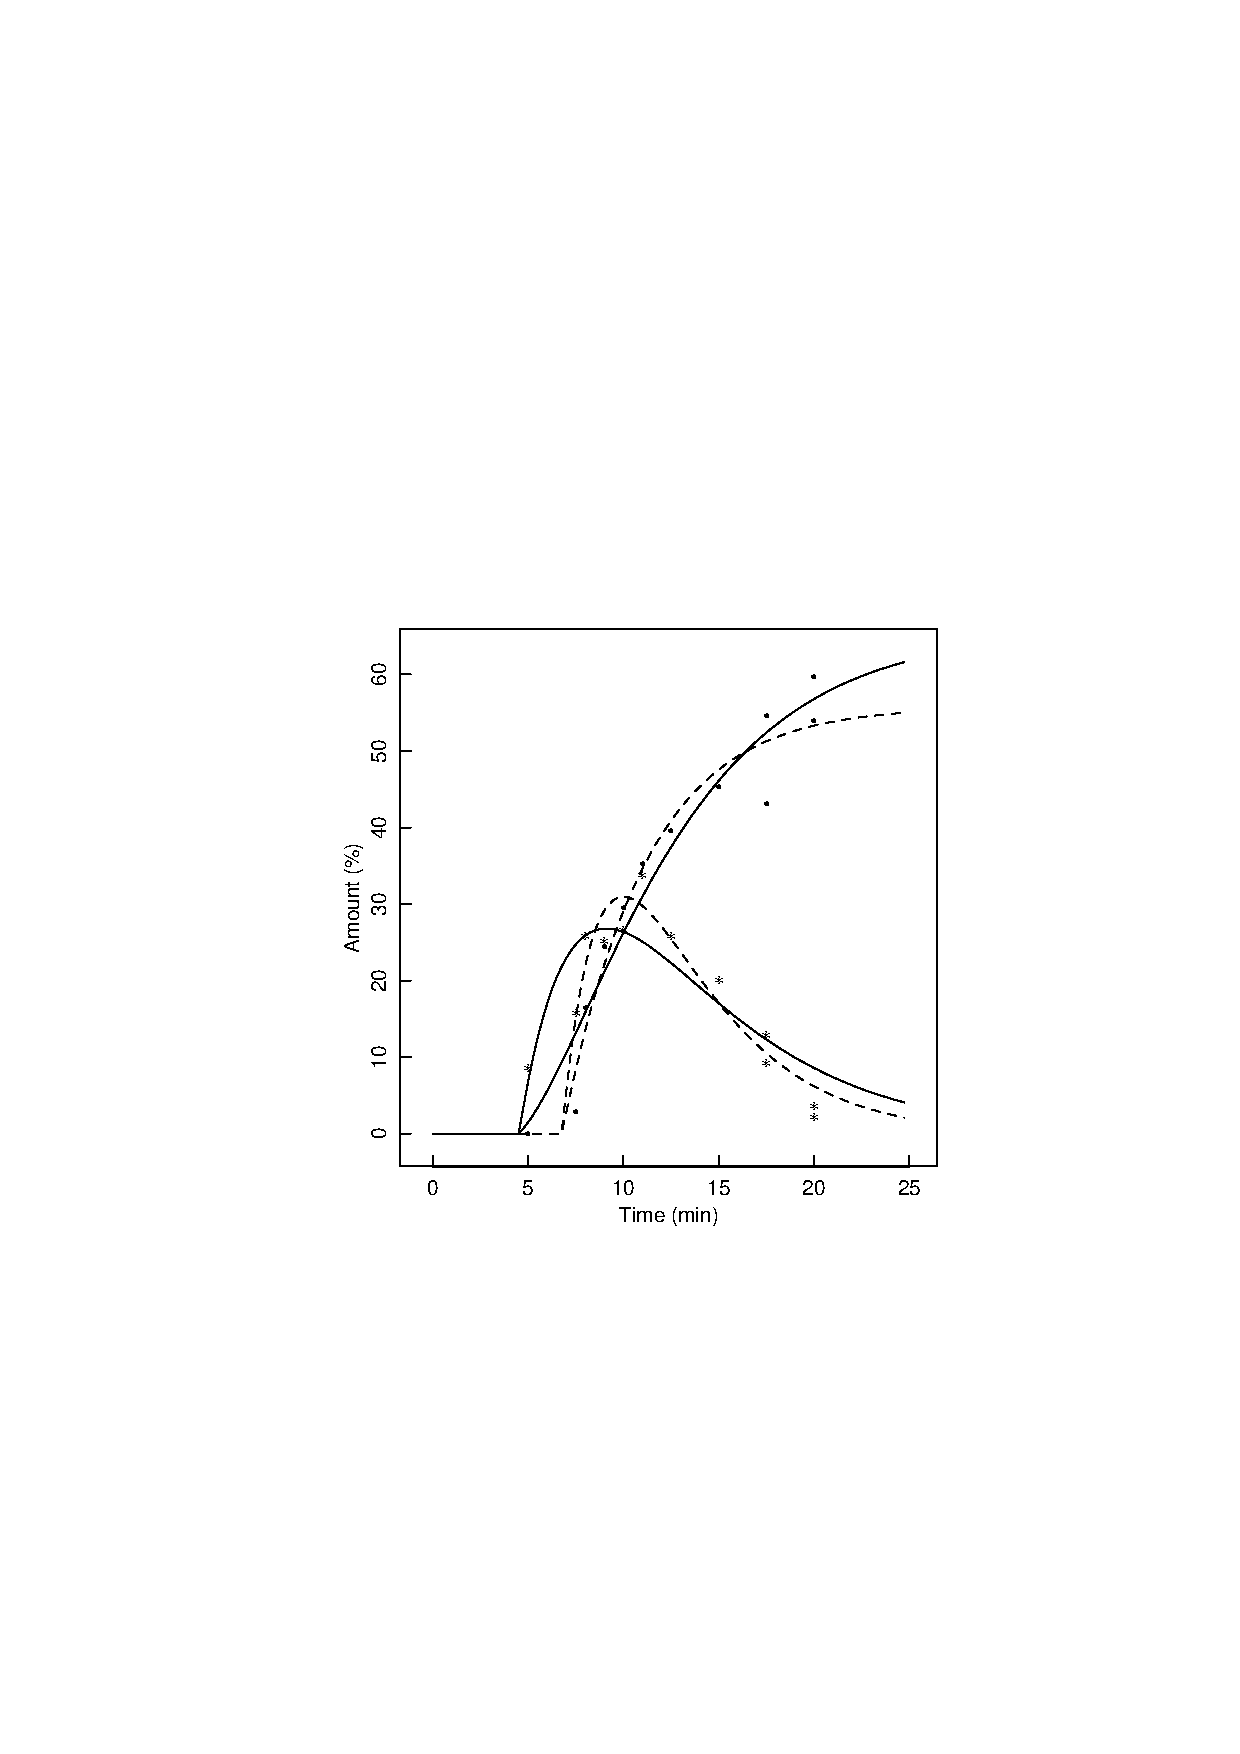
\includegraphics{5OIL450pred}}%,height=4in}}
  \caption{\label{fig:OIL450pred}
  Plot of oil ($\bullet$) and bitumen ($*$) amounts versus time for the
  temperatures for the oil shale data at 723K.
  The fitted curves for a dead time of 4.5 minutes are shown as solid
  lines, and the fitted curves for a dead time of 6.8 minutes are shown as
  dashed lines.
  }
\end{figure}
reveals that a tradeoff is being made:
the oil concentration is best fitted with a dead time 6.8
minutes, while the bitumen concentration is best fitted with a
dead time of 4.5 minutes.
The optimum with the larger dead time has a smaller
determinant, but from the plots and from consideration of the
data at other temperatures, it appears that the predictions
with the smaller dead time are better.

Individual fits were made to the data at the remaining temperatures
and are recorded in
Table~\ref{tbl:alltemp}.
\begin{table}
  \caption{\label{tbl:alltemp}
  Parameter summary for the oil shale data at all temperatures together
  with the scaled inverse temperature variable and the parameters
  from a linear regression of each kinetic parameter on scaled inverse
  temperature.
  }
  \begin{tabular}{l r r r r r}
    %c c c c c c c
    %c c c c c c c
    %c n n n n n n.
    %\par\vspace{2.0pt}
    %\_
    %Temperature
    %(K)*$ln\theta_1 $*$ln\theta_2 $*
    %$ln\theta_3 $*$ln\theta_4 $*$t_{0}$*$T_{ {\rm inv} }$
    %\_
    %673*--4.064*--4.720*--3.912*--4.557*7.771*--\/0.0517
    %698*--2.546*--3.051*--2.975*--3.694*6.247*--\/0.0249
    %723*--1.835*--1.889*--2.283*--3.610*4.526*0.0000
    %748*--\/0.801*--1.252*--1.264*--2.082*4.082*0.0233
    %773*--\/0.447*--\/0.853*--\/0.803*--1.623*2.938*0.0450
    %798*0.287*--\/0.120*--\/0.297*--\/0.998*2.849*0.0654
    %\_
    %%.T&
    %l n n n n n n.
    %Intercept:*--1.907*--2.335*--2.221*--3.056*5.146
    %Slope:*35.73*37.27*31.37*31.09*--43.14
    %\_
  \end{tabular}
\end{table}

\subsection{Starting Estimates for the Process Parameters}

To get starting estimates for the process parameters in the
Arrhenius relation, we introduced the negative scaled inverse
temperature variable
$$
T_{\mbox{\rm inv} } = {-1000  \over 1.987 }\left( {1 \over T}-{1\over 723}\right)
$$
which centers about the middle temperature 723 K and
includes a factor of 1000 to convert
the units of the activation energy from cal/g-mole to the more
convenient kcal/g-mole.
The negative sign is used so that increasing $T$ increases
$T_{\mbox{\rm inv}}$.

The slopes and intercepts from linear regressions of each
kinetic parameter on $T_{\mbox{\rm inv}}$, included in Table~\ref{tbl:alltemp},
were used as starting estimates for the scaled
preexponential and activation energies in the Arrhenius model.
A plot of dead time versus $T_{\mbox{\rm inv}}$ indicated that a linear
model for $t_{0}$ versus $T_{\mbox{\rm inv}}$ was also reasonable.

\subsection{Fitting the Complete Data Set}

We simultaneously fitted
the data for both responses at all six temperatures to a model with ten
process parameters, consisting of
four rate constants (i.e., preexponential terms)
and the dead time $t_{0}$ at 723 K, plus
four activation energies and the slope of $t_{0}$ versus $T_{\mbox{\rm inv}}$.

The final parameter summary is given in
Table~\ref{tbl:process}.
\begin{table}
  \caption{\label{tbl:process}
  Parameter summary for the complete oil shale data set.
  }
  \begin{tabular}{l r r r r r}
    %.sz 8
    %c  c c c s s s s s s s s
    %c  c c c s s s s s s s s
    %c  c c c s s s s s s s s
    %c  n n n 1 n 1 n 1 n 1 n 1 n 1 n 1 n 1 n.
    %\_
    %::Approx.
    %::Std.
    %:Est.:Error:Approximate Correlation Matrix
    %\par\vspace{2.0pt}
    %\_
    %$\phi_{1}$:--1.920:0.079:1.00
    %$\phi_{2}$:--2.277:0.127:0.38:1.00
    %$\phi_{3}$:--2.195:0.076:0.52:0.09:1.00
    %$\phi_{4}$:--3.024:0.164:--\/0.02:--\/0.84:0.25:1.00
    %$t_{0}$:4.406:0.227:0.50:--\/0.15:0.44:0.52:1.00
    %$E_{1}$:38.14:1.956:0.08:--\/0.12:0.03:0.19:0.19:1.00
    %$E_{2}$:34.25:3.303:--\/0.06:--\/0.17:--\/0.02:0.07:0.00:0.54:1.00
    %$E_{3}$:34.41:1.848:0.01:--\/0.07:--\/0.16:0.10:0.14:0.45:0.30:1.00
    %$E_{4}$:36.13:3.864:0.18:0.02:0.10:0.16:0.21:--\/0.25:--\/0.84:0.01:1.00
    %$\beta$:--24.67:3.311:--\/0.43:0.13:--\/0.39:--\/0.45:--\/0.96:--\/0.08:--\/0.01:--\/0.07:--\/0.12
    %\_
  \end{tabular}
\end{table}
Estimates of each of the kinetic parameters from the individual
temperature data are plotted versus $T_{\mbox{\rm inv}}$ in
Figure~\ref{fig:OILlogk}
\begin{figure}
  \centerline{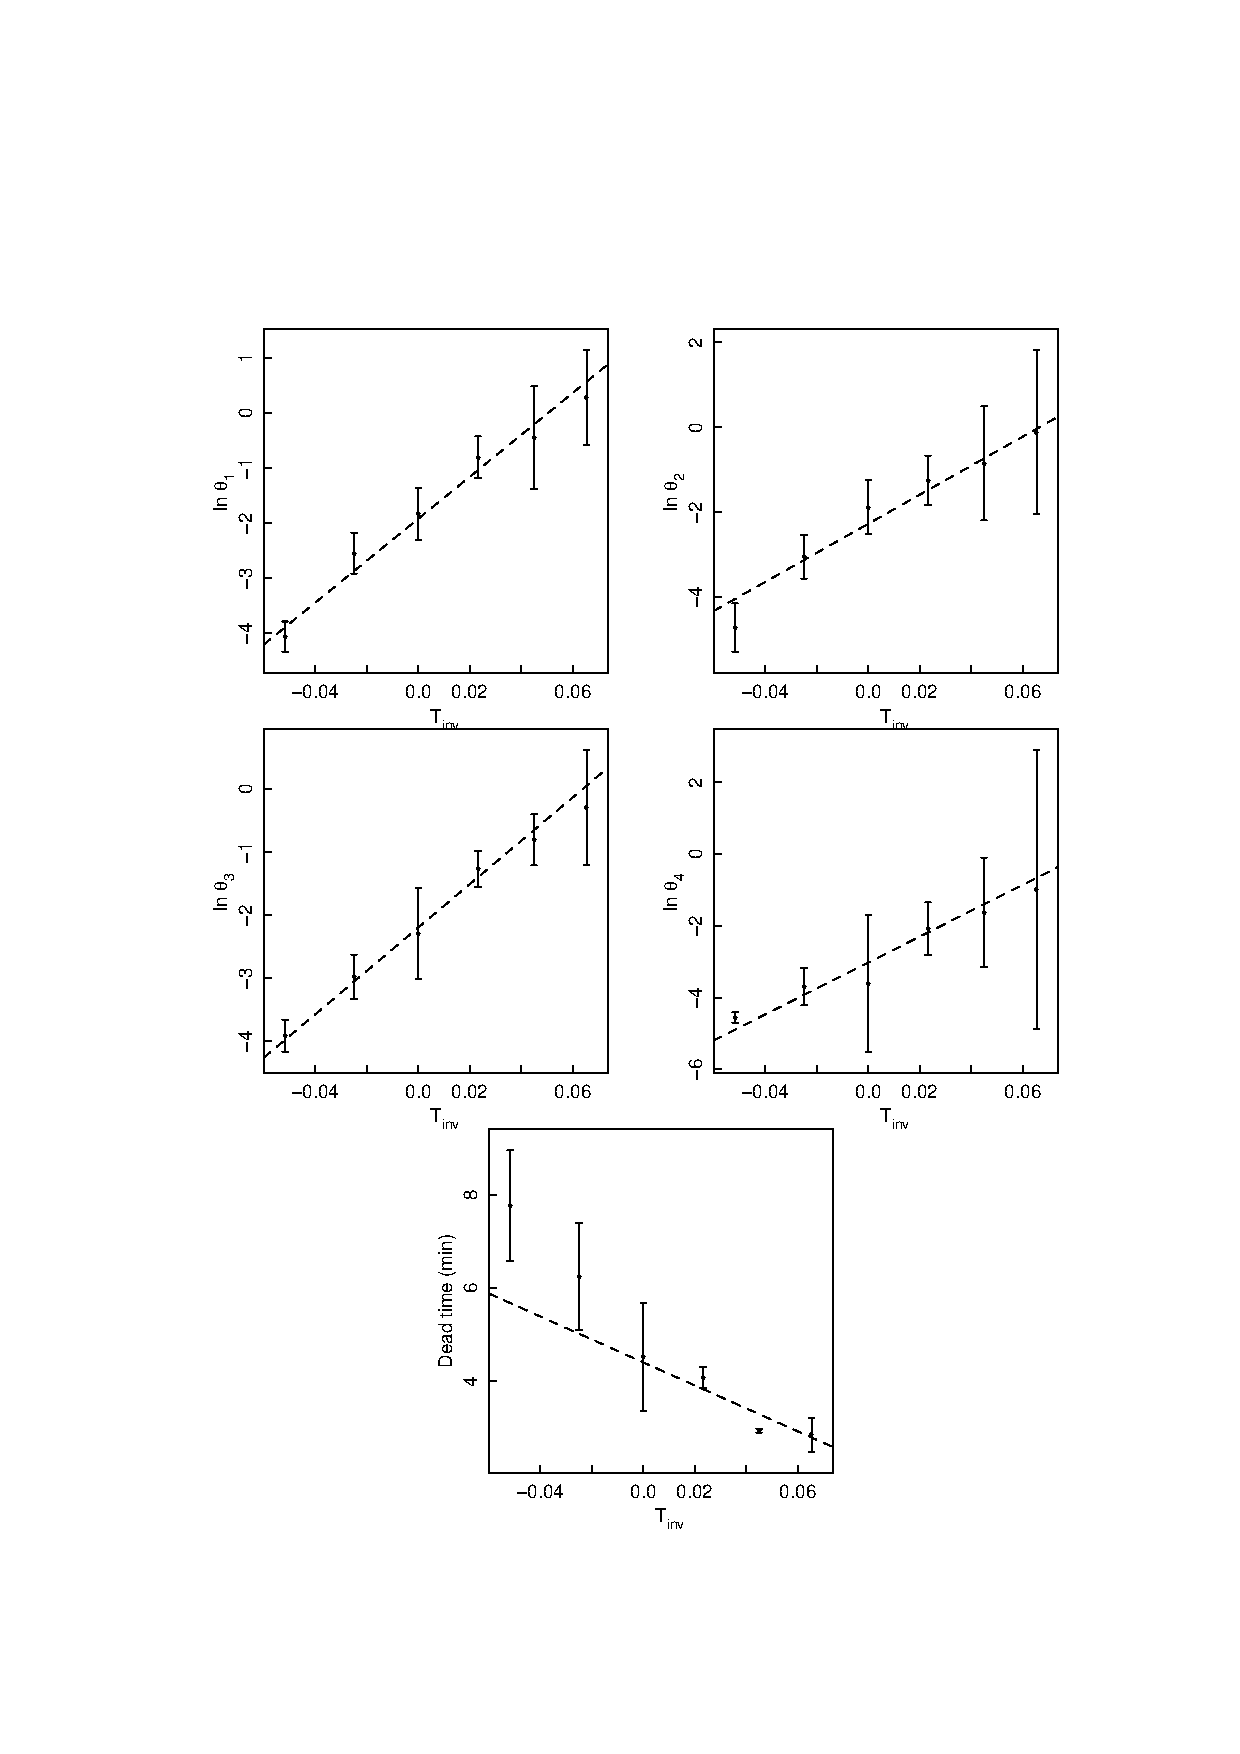
\includegraphics{5OILlogk}}%,width=\textwidth}}
  \caption{\label{fig:OILlogk}
  Plots of kinetic parameter estimates and Arrhenius model fits for
  the oil shale data.  The kinetic parameter estimates and their
  approximate 95\% inference intervals are shown as solid lines.  The
  Arrhenius model fits are shown as dashed lines.
  }
\end{figure}
together with the estimated Arrhenius relation from the process model.
Each of the individual estimates is shown with bars representing
approximate 95\% HPD intervals.
The process model for $t_{0}$ does not appear to follow the individual
estimates well, but we note that $t_{0}$ is much more
precisely determined at higher values of $T_{{{\rm }} inv }$,
where the Arrhenius relation fits the data well.
Plots of the fitted curves versus time are overlaid with the
original data in Figure~\ref{fig:OILpred}.
\begin{figure}
  \centerline{
\includegraphics{5OILpred}}%,width=\textwidth}}
  \caption{\label{fig:OILpred}
  Plot of oil ($\bullet$) and bitumen ($*$) amounts versus time
  for six temperatures for the oil shale pyrolysis data together with
  the fitted curves.  The fitted curves for oil are shown as dashed
  lines, and those for bitumen as solid lines.
  }
\end{figure}
For low temperatures and early times, the model does not fit well.

\subsection{Conclusions}

We have fitted the process model to the multiresponse data over a
range of temperatures.
The fitted parameters have reasonable values, and the assumptions
on the disturbances do not appear inappropriate.
However, the assumed kinetic model does have deficiencies, and so we
should consult experts on chemical kinetics to try to formulate
a better model.
One obvious change in the model is to allow for different dead times
for bitumen and for oil, with
$t_0^{\mbox{\rm oil}}>t_0^{\mbox{\rm bitumen}}$.

\begin{problems}

  \prob 

  \subprob Write a computer routine in a language of your choice to
  solve systems of linear differential equations, using the pseudocode
  of Appendix 3, Section A3.4.  Assume that the transfer matrix $\bA$
  is diagonalizable.

  \subprob Extend the subroutine to evaluate derivatives of the
  expectation functions with respect to the parameters for bolus and
  step inputs.

  \prob

  \subprob 
  Show that the system matrix $\bA$ for the chemical reaction
  with system diagram
  \expandafter\ifx\csname graph\endcsname\relax \csname newbox\endcsname\graph\fi
\expandafter\ifx\csname graphtemp\endcsname\relax \csname newdimen\endcsname\graphtemp\fi
\setbox\graph=\vtop{\vskip 0pt\hbox{%
    \special{pn 8}%
    \special{ar 250 250 250 250 0 6.28319}%
    \graphtemp=.5ex\advance\graphtemp by 0.250in
    \rlap{\kern 0.250in\lower\graphtemp\hbox to 0pt{\hss $\gamma_{1}$\hss}}%
    \special{ar 1250 250 250 250 0 6.28319}%
    \graphtemp=.5ex\advance\graphtemp by 0.250in
    \rlap{\kern 1.250in\lower\graphtemp\hbox to 0pt{\hss $\gamma_{2}$\hss}}%
    \special{pa 500 250}%
    \special{pa 1000 250}%
    \special{fp}%
    \special{sh 1.000}%
    \special{pa 900 225}%
    \special{pa 1000 250}%
    \special{pa 900 275}%
    \special{pa 900 225}%
    \special{fp}%
    \graphtemp=\baselineskip\multiply\graphtemp by -1\divide\graphtemp by 2
    \advance\graphtemp by .5ex\advance\graphtemp by 0.250in
    \rlap{\kern 0.750in\lower\graphtemp\hbox to 0pt{\hss $\theta_{1}$\hss}}%
    \special{pa 250 500}%
    \special{pa 250 1000}%
    \special{fp}%
    \special{sh 1.000}%
    \special{pa 275 900}%
    \special{pa 250 1000}%
    \special{pa 225 900}%
    \special{pa 275 900}%
    \special{fp}%
    \graphtemp=.5ex\advance\graphtemp by 0.750in
    \rlap{\kern 0.250in\lower\graphtemp\hbox to 0pt{\hss $\theta_{2}$ }}%
    \hbox{\vrule depth1.000in width0pt height 0pt}%
    \kern 1.500in
  }%
}%

  \centerline{\box\graph}
  has eigenvalues $( - ( \theta_1+\theta_2 ) ,0 ) \trans$ and
  eigenvectors
  $$
  \bU=\left[ \matrix {
      \matrix{{\theta_1 +\theta_2} \cr {- \theta_1}}
      \matrix{0 \cr 1}
    }\right]
  $$
  with
  $$
  \bU^{-1}=\left[
    \begin{array}{c c}
      1/(\theta_1+\theta_2)&0\\
      \theta_1/(\theta_1+\theta_2)&1
    \end{array}\right]
  $$

  \subprob Use the results from part (a) to show that the response at
  time $t$ to an initial concentration of 100\% in response 1 and 0\%
  concentration in response 2 is
  $$
  \bgamma( t )=\left[ \matrix{
      \matrix {e^{{-} ( \theta_1 +\theta_2 )t} \cr
        {\theta_1 \over \theta_1 +\theta_2}
        \left( 1-e^{{-} ( \theta_1 +\theta_2 )t}\right)}
    }\right]
  $$

  \prob Use the data from Appendix 4, Section A4.8 to fit a
  compartment model.

  \prob

  \subprob Use the results from Example Tetracycline 5 to derive the
  derivatives of the model function with respect to the parameters.
  \subprob Verify that the derivatives in part (a) are correct by
  differentiating the explicit solutions for the functions given in
  Example Tetracycline 3.

  \prob Use a multiresponse parameter estimation criterion to fit the
  model from Example $\alpha$-pinene 2, to the
  $\alpha$-pinene data at 204.5$^\circ$C given in Appendix 4,
  Section A4.6.

  \subprob Use the method of Section 4.3 to determine starting values.

  \subprob Use an extra determinant analysis to decide whether the path
  from allo-ocimene to pyronene is necessary.
  
\end{problems}

% Local Variables: 
% mode: latex
% TeX-master: "nraia2"
% End: 
